\documentclass[12pt,a4paper]{extarticle}
\usepackage[top=1cm,bottom=1cm,left=2cm,right=2cm]{geometry}
\renewcommand{\familydefault}{\sfdefault}
\usepackage[utf8]{inputenc}
\usepackage{lastpage}
\usepackage{hyperref}
\usepackage{anyfontsize}
\usepackage{float}
\usepackage{alphalph}
\usepackage{lipsum}
\usepackage{graphicx} 
\usepackage{blindtext}
\usepackage{framed}
\usepackage{enumitem}
\usepackage{soul}
\usepackage{subcaption}
\usepackage{lmodern}
\usepackage{wrapfig}
\usepackage{textcomp}
\usepackage{xstring}
\usepackage{xcolor}
\usepackage{tikz}
\usetikzlibrary{shapes,arrows,positioning, calc}
\usepackage[labelformat=empty,hypcap=false]{caption}
\usepackage{fancyhdr}
\usepackage[lastpage]{zref}
\usepackage{array}
\newcolumntype{L}[1]{>{\raggedright\arraybackslash}p{#1}}
\newcolumntype{R}[1]{>{\raggedleft\arraybackslash}p{#1}}
\newcolumntype{C}[1]{>{\centering\arraybackslash}p{#1}}

\renewcommand{\thefootnote}{\arabic{footnote}}

\newlength\q
\setlength\q{\dimexpr .363\textwidth -4\tabcolsep}

\newcommand{\drawBar}[1]{
\begin{minipage}[c][0.5cm][c]{1.0\textwidth}
    \hspace*{-0.75cm} 
    \ifodd\thepage\else\hfill\fi
    \textbf{\thepage} / \textbf{\reallastpage}
    \ifodd\thepage\else\hspace*{0.55cm}\fi
\end{minipage}
}

\newcommand{\drawParagraph}[1]{
\paragraph{#1} \texttt{ } \newline
}

\newcommand{\createlabel}[2]{%
    \expandafter\edef\csname#1\endcsname{#2}
}

\newcommand{\EenSpeler}{\textbf{[Een speler] }}
\newcommand{\EenSpelerN}{\textbf{[Een speler]}}

\newcommand{\eenSpeler}{\textbf{[een speler] }}
\newcommand{\eenSpelerN}{\textbf{[een speler]}}

\newcommand{\huidigeSpeler}{\textbf{[huidige speler] }}
\newcommand{\huidigeSpelerN}{\textbf{[huidige speler]}}

\newcommand{\HuidigeSpeler}{\textbf{[Huidige speler] }}
\newcommand{\HuidigeSpelerN}{\textbf{[Huidige speler]}}

\newcommand{\andereSpeler}{\textbf{[andere speler] }}
\newcommand{\andereSpelerN}{\textbf{[andere speler]}}

\newcommand{\AndereSpeler}{\textbf{[Andere speler] }}
\newcommand{\AndereSpelerN}{\textbf{[Andere speler]}}

\newcommand{\andereSpelers}{\textbf{[andere spelers] }}
\newcommand{\andereSpelersN}{\textbf{[andere spelers]}}

\newcommand{\AndereSpelers}{\textbf{[Andere spelers] }}
\newcommand{\AndereSpelersN}{\textbf{[Andere spelers]}}

\newcommand{\alleSpelers}{\textbf{[alle spelers]} }
\newcommand{\alleSpelersN}{\textbf{[alle spelers]}}

\newcommand{\AlleSpelers}{\textbf{[Alle spelers] }}
\newcommand{\AlleSpelersN}{\textbf{[Alle spelers]}}

\newcommand{\MedeSpeler}{\textbf{[Medespeler] }}
\newcommand{\MedeSpelerN}{\textbf{[Medespeler]}}

\newcommand{\medeSpeler}{\textbf{[medespeler]} }
\newcommand{\medeSpelerN}{\textbf{[medespeler]}}

\newcommand{\MedeSpelers}{\textbf{[Medespelers] }}
\newcommand{\MedeSpelersN}{\textbf{[Medespelers]}}

\newcommand{\medeSpelers}{\textbf{[medespelers]} }
\newcommand{\medeSpelersN}{\textbf{[medespelers]}}

\newcommand{\VorigeSpeler}{\textbf{[Vorige speler] }}
\newcommand{\VorigeSpelerN}{\textbf{[Vorige speler]}}

\newcommand{\vorigeSpeler}{\textbf{[vorige speler] }}
\newcommand{\vorigeSpelerN}{\textbf{[vorige speler]}}

\newcommand{\VolgendeSpeler}{\textbf{[Volgende speler] }}
\newcommand{\VolgendeSpelerN}{\textbf{[Volgende speler]}}

\newcommand{\volgendeSpeler}{\textbf{[volgende speler] }}
\newcommand{\volgendeSpelerN}{\textbf{[volgende speler]}}

\newcommand{\deSpeler}{\textbf{[de speler] }}
\newcommand{\deSpelerN}{\textbf{[de speler]}}

\newcommand{\DeSpeler}{\textbf{[De speler] }}
\newcommand{\DeSpelerN}{\textbf{[De speler]}}

\newcommand{\Willem}{\textbf{[Willem] }}
\newcommand{\WillemN}{\textbf{[Willem]}}

\newcommand{\Frits}{\textbf{[Frits] }}
\newcommand{\FritsN}{\textbf{[Frits]}}

\newcommand{\Lisa}{\textbf{[Lisa] }}
\newcommand{\LisaN}{\textbf{[Lisa]}}

\newcommand{\Kim}{\textbf{[Kim] }}
\newcommand{\KimN}{\textbf{[Kim]}}

\newcommand{\Fritsen}{\textbf{Fritsen} }
\newcommand{\FritsenN}{\textbf{Fritsen}}

\newcommand{\customBox}[1]{
    \begin{framed}
    \noindent
    #1
    \end{framed}
}

\newcommand{\customBoxItalic}[1]{
    \begin{framed}
    \noindent
    \textit{#1}
    \end{framed}
}


\newcommand{\kaart}[1]{\textbf{\ul{#1}}}

\newcommand{\hoofdstuk}[2]{\vspace{-0.5cm}\section*{#1. #2}}
\newcommand{\deelhoofdstuk}[1]{\vspace{-0.5cm}\noindent\subsection*{#1}}

\newcommand{\beginLijst}[1]{
    \def \sectieNummer {#1}
    \begin{enumerate}[label=\texttt{\sectieNummer-\arabic*},align=left, labelwidth=31pt, leftmargin=37pt]
}

\newcommand{\vervolgLijst}[0]
    {\begin{enumerate}[label=\texttt{\sectieNummer-\arabic*},resume,align=left, labelwidth=31pt, leftmargin=37pt]
}

\newcommand{\beginLijstKlein}[1]{
    \def \sectieNummer {#1}
    \begin{enumerate}[label=\texttt{\sectieNummer-\arabic*},align=left, labelwidth=21pt, leftmargin=27pt]
}

\newcommand{\vervolgLijstKlein}[0]
    {\begin{enumerate}[label=\texttt{\sectieNummer-\arabic*},resume,align=left, labelwidth=21pt, leftmargin=27pt]
}

\newcommand{\numeriekeLijst}[0]
    {\begin{enumerate}[label=\arabic*.,nolistsep]
}

\newcommand{\eindNumeriekeLijst}[0]{
    \end{enumerate}
}

\newcommand{\beginABCLijst}[1]{
    \def \sectieNummer {#1}
    \begin{enumerate}[label=\texttt{\sectieNummer\Alph*},nolistsep,align=left, labelwidth=25pt, leftmargin=31pt]
}

\newcommand{\beginABCLijstKlein}[1]{
    \def \sectieNummer {#1}
    \begin{enumerate}[label=\texttt{\sectieNummer\Alph*},nolistsep,align=left, labelwidth=13pt, leftmargin=19pt]
}


\newcommand{\eindABCLijst}[0]{
    \end{enumerate}
}

\newcommand{\puntLijst}[0]{
    \begin{itemize}[label=$\circ$,nolistsep]
}

\newcommand{\eindPuntLijst}[0]{
    \end{itemize}
}

\newcommand{\eindLijst}[0]{
    \end{enumerate}
}

\newcommand{\quotes}[1]{\textquotedblleft\textit{#1}\textquotedblright}

\setlength\tabcolsep{0pt}
\newcommand{\kaartnaam}[5]{
\begin{minipage}[c][2.25cm][c]{1.0\textwidth}
    \begin{tabularx}{\textwidth}{Xccccm{0.00cm}}
        \vspace{-1.6cm}
        \begin{flushleft}
            #1
        \end{flushleft}&
        \ifx&#2&%
            &
        \else
            \includegraphics[height=2cm]{img/cards/generated/#2.png} \hspace{0.05cm} &
        \fi
        \ifx&#3&%
            &
        \else
            \includegraphics[height=2.0cm]{img/cards/generated/#3.png} \hspace{0.05cm} &
        \fi
        \ifx&#4&%
            &
        \else
            \includegraphics[height=2.0cm]{img/cards/generated/#4.png} \hspace{0.05cm} &
        \fi
        \ifx&#5&%
            &
        \else
            \includegraphics[height=2.0cm]{img/cards/generated/#5.png} &
        \fi
    \end{tabularx}
\end{minipage}
}

\newcommand{\zetKort}[8]{
\deelhoofdstuk{#1}
    \noindent
    \begin{tikzpicture}
        \def\h{2.5}
        \node (img1) {\includegraphics[height=\h cm]{img/cards/generated/#2.png}};
        \node (img2) at (img1.south east) [xshift=-\h*0.29cm,yshift=\h*0.455cm] {\includegraphics[height=\h cm]{img/cards/generated/#3.png}};
    \end{tikzpicture}
    \begin{tikzpicture}
        \def\h{2.5}
        \node (img1) {\includegraphics[height=\h cm]{img/cards/generated/#4.png}};
        \node (img2) at (img1.south east) [xshift=-\h*0.29cm,yshift=\h*0.455cm] {\includegraphics[height=\h cm]{img/cards/generated/#5.png}};
    \end{tikzpicture}
    \begin{tikzpicture}
        \def\h{2.5}
        \node (img1) {\includegraphics[height=\h cm]{img/cards/generated/#6.png}};
        \node (img2) at (img1.south east) [xshift=-\h*0.29cm,yshift=\h*0.455cm] {\includegraphics[height=\h cm]{img/cards/generated/#7.png}};
    \end{tikzpicture}
    \newline
    #8
}

\newcommand{\zetKoningAas}[5]{
    \noindent
    \begin{minipage}[t][3.5cm][t]{1.0\textwidth}
        \begin{wrapfigure}{L}{10.9cm}
            \vspace{-15pt}
            \begin{tikzpicture}
                \def\h{2.4}
                \node (img1) {\includegraphics[height=\h cm]{img/cards/generated/queen_of_#1.png}};
                \node (img2) at (img1.south east) [xshift=-\h*0.27cm,yshift=\h*0.455cm] {\includegraphics[height=\h cm]{img/cards/generated/king_of_#1.png}};
                \node (img3) at (img2.south east) [xshift=-\h*0.27cm,yshift=\h*0.555cm] {\includegraphics[height=\h cm]{img/cards/generated/ace_of_#1.png}};
            \end{tikzpicture}
            \begin{tikzpicture}
                \def\h{2.4}
                \node (img1) {\includegraphics[height=\h cm]{img/cards/generated/queen_of_#2.png}};
                \node (img2) at (img1.south east) [xshift=-\h*0.27cm,yshift=\h*0.455cm] {\includegraphics[height=\h cm]{img/cards/generated/king_of_#2.png}};
                \node (img3) at (img2.south east) [xshift=-\h*0.27cm,yshift=\h*0.555cm] {\includegraphics[height=\h cm]{img/cards/generated/ace_of_#2.png}};
            \end{tikzpicture}
            \begin{tikzpicture}
                \def\h{2.4}
                \node (img1) {\includegraphics[height=\h cm]{img/cards/generated/queen_of_#3.png}};
                \node (img2) at (img1.south east) [xshift=-\h*0.27cm,yshift=\h*0.455cm] {\includegraphics[height=\h cm]{img/cards/generated/king_of_#3.png}};
                \node (img3) at (img2.south east) [xshift=-\h*0.27cm,yshift=\h*0.555cm] {\includegraphics[height=\h cm]{img/cards/generated/ace_of_#32.png}};
            \end{tikzpicture}
            \begin{tikzpicture}
                \def\h{2.4}
                \node (img1) {\includegraphics[height=\h cm]{img/cards/generated/queen_of_#4.png}};
                \node (img2) at (img1.south east) [xshift=-\h*0.27cm,yshift=\h*0.455cm] {\includegraphics[height=\h cm]{img/cards/generated/king_of_#4.png}};
                \node (img3) at (img2.south east) [xshift=-\h*0.27cm,yshift=\h*0.555cm] {\includegraphics[height=\h cm]{img/cards/generated/ace_of_#4.png}};
            \end{tikzpicture}
        \end{wrapfigure}
        #5.
    \end{minipage}
}

\newcommand{\zetLangMetKruis}[9]{
    \noindent
    \begin{minipage}[t][#1cm][t]{1.0\textwidth}
        \begin{wrapfigure}{L}{5.0cm}
            \vspace{-15pt}
            \begin{tikzpicture}
                \def\h{2.5}
                \node (img1) {\includegraphics[height=\h cm]{img/cards/generated/#2.png}};
                \node (img2) at (img1.south east) [xshift=-\h*0.27cm,yshift=\h*0.455cm] {\includegraphics[height=\h cm]{img/cards/generated/#3.png}};
            \end{tikzpicture}
            \begin{tikzpicture}
                \def\h{2.5}
                \node (img1) {\includegraphics[height=\h cm]{img/cards/generated/#4.png}};
                \node (img2) at (img1.south east) [xshift=-\h*0.27cm,yshift=\h*0.455cm] {\includegraphics[height=\h cm]{img/cards/generated/#5.png}};
                
                \draw [red,ultra thick,rounded corners]([xshift=\h*0.04cm,yshift=-\h*0.04cm]img1.north west) -- ([xshift=-\h*0.04cm,yshift=\h*0.04cm]img2.south east);
                \draw [red,ultra thick,rounded corners]([xshift=-\h*0.04cm,yshift=\h*0.05cm]img2.north east) -- ([xshift=-\h*0.085cm,yshift=\h*0.04cm]img2.south west);   
            \end{tikzpicture}
        \end{wrapfigure}
        #6: 
        \ifx&#7&%
        \else
            \ifx&#8&%
                \begin{itemize}[nolistsep,leftmargin=*]
                    \item #7
                \end{itemize}       
            \else
                \begin{itemize}[nolistsep,leftmargin=*]
                    \item #7
                    \item #8
                \end{itemize}
            \fi
        \fi
        \ifx&#9&%
        \else
            \ifx&#7&%
                \newline
                #9
            \else
                #9
            \fi
        \fi
    \end{minipage}
}

\newcommand{\zetLang}[9]{
    \noindent
    \begin{minipage}[t][#1cm][t]{1.0\textwidth}
        \begin{wrapfigure}{L}{5.0cm}
            \vspace{-15pt}
            \begin{tikzpicture}
                \def\h{2.5}
                \node (img1) {\includegraphics[height=\h cm]{img/cards/generated/#2.png}};
                \node (img2) at (img1.south east) [xshift=-\h*0.27cm,yshift=\h*0.455cm] {\includegraphics[height=\h cm]{img/cards/generated/#3.png}};
            \end{tikzpicture}
            \begin{tikzpicture}
                \def\h{2.5}
                \node (img1) {\includegraphics[height=\h cm]{img/cards/generated/#4.png}};
                \node (img2) at (img1.south east) [xshift=-\h*0.27cm,yshift=\h*0.455cm] {\includegraphics[height=\h cm]{img/cards/generated/#5.png}}; 
            \end{tikzpicture}
        \end{wrapfigure}
        #6: 
        \ifx&#7&%
        \else
            \ifx&#8&%
                \begin{itemize}[nolistsep,leftmargin=*]
                    \item #7
                \end{itemize}       
            \else
                \begin{itemize}[nolistsep,leftmargin=*]
                    \item #7
                    \item #8
                \end{itemize}
            \fi
        \fi
        \ifx&#9&%
        \else
            \ifx&#7&%
                \newline
                #9
            \else
                #9
            \fi
        \fi
    \end{minipage}
}

\newcommand{\proLabel}[0]{
    \hspace{-0.25cm}\tcbox{\textit{\textcolor{white}{PRO}}}
}

\newcommand{\proLabelMetRuimte}[0]{
    \tcbox{\textit{\textcolor{white}{PRO}}}
}

\newcommand{\tweedeDruk}[0]{
\begingroup
    \fontsize{30pt}{36pt}\selectfont
    \tcbox{\textit{\textcolor{white}{2\hspace*{0.1cm}\textsuperscript{e} druk}}}
\endgroup
}




\def\Put(#1,#2)#3{\leavevmode\makebox(0,0){\put(#1,#2){#3}}}

\usepackage[export]{adjustbox}
\usepackage{array}
\usepackage{tabularx}
\usepackage{comment}
\usepackage{twemojis}
\usepackage{scalerel}
\usepackage{svg}
\usepackage[absolute,overlay]{textpos}

\usepackage[most]{tcolorbox}
\tcbset{on line, 
        boxsep=4pt, left=0pt,right=0pt,top=0pt,bottom=0pt,
        colframe=white,colback=black,  
        highlight math style={enhanced}
        }


\setuldepth{Berlin}

\makeatletter
\newcommand{\reallastpage}{%
  \the\numexpr\zref@extractdefault{LastPage}{page}{0}-1\relax
}



\renewcommand*{\@Alph}[1]{%
  \ifcase#1\or A\or B\or C\or
    D\or E\or F\or G\or H\or I\or J\or
    K\or L\or M\or N\or O\or P\or R\or S\or
    T\or U\or V\or W\or X\or
    Y\or Z\or AA\or AB\or AC\or
    AD\or AE\or AF\or AG\or AH\or AI\or AJ\or
    AK\or AL\or AM\or AN\or AO\or AP\or AR\or AS\or
    AT\or AU\or AV\or AW\or AX\or
    AY\or AZ \else\@ctrerr\fi
}
\makeatother

\begin{document}

%\fontsize{50}{60}\selectfont Foo
\thispagestyle{empty}
\begingroup
    \fontsize{80pt}{82pt}\selectfont
    \begin{center}
        Fritsen in 2023  
    \end{center}
\endgroup

\vspace{0.55cm}

\begin{center}
    
\includegraphics[width=10cm]{bier.jpeg}
\end{center}

\begingroup
    \fontsize{80pt}{82pt}\selectfont
    \begin{center}
        Spelregels  
    \end{center}
\endgroup

\vspace{0.1cm}

\begingroup
    \fontsize{30pt}{32pt}\selectfont
    \begin{center}
        \texttt{Met de eerste drie pagina's \\en de achterkant van dit document kun je al Fritsen}
    \end{center}
\endgroup

\newpage

\setcounter{page}{1}
\pagestyle{fancy}

\fancyhf{}
\renewcommand{\headrulewidth}{0pt}
%\fancyhead[L]{
%\begin{tabular}[t]{l}
%    1. Definities (p. 3)\\ 4. Uitspraken (p. 12)
%\end{tabular}
%}
%\fancyhead[C]{
%\begin{tabular}[t]{l}
%    2. Regels (p. 4 t/m 11)\\ 5. Varianten (p. 12)
%\end{tabular}
%}
%\fancyhead[R]{
%\begin{tabular}[t]{l}
%    3. Kaartnamen (p. 12)\\ 6. Zetten (p. 13 t/m 14)
%\end{tabular}
%}
 
\setlength{\headsep}{0.9cm}




  
\drawBar{Introductie}
\vspace{-0.5cm}
\section*{Introductie}
\drawParagraph{Het spel in het kort}
$-$ Fritsen is een drankspel met kaarten dat gespeeld wordt met minimaal 2 en maximaal 10 personen. \newline $-$ Om de beurt leg je een kaart neer en moet er mogelijk gedronken worden. \newline $-$ Als je \ul{\texttt{ADTEN}} zegt moet je proosten op \quotes{Frits} en een shotglaasje bier drinken. 
\vspace*{-0.22cm} 

\drawParagraph{Doel van het spel} 
$-$ Al je kaarten in zo weinig mogelijk zetten wegleggen.

\vspace*{-0.22cm} 

\drawParagraph{Geschatte speelduur}
$-$ 15 tot 45 minuten.

\vspace*{-0.22cm} 

\drawParagraph{Benodigdheden}
$-$ Voldoende bier, shotglaasjes en een snijplank voor de kaarten. \newline $-$ Tot en met 6 personen \ul{\'e\'en} pak kaarten en voor meer dan 6 personen \ul{twee} pakken kaarten.

\vspace*{-0.22cm} 

\drawParagraph{Speelbord}
$-$ \'E\'en \ul{dichte} stapel kaarten, \'e\'en \ul{open} jokerstapel en meerdere \ul{open} stapels voor niet-jokers.

\noindent\rule{\textwidth}{1pt}
\centerline{\textit{"\Fritsen of \textbf{een Fritsje nemen} is het drinken van één shotglaasje bier."}} \\
\centerline{\textit{"\textbf{Dubbelfritsen} of \textbf{een dubbele Frits nemen} is het drinken van twee shotglaasjes bier."}} \vspace*{-0.7cm}  \\
\noindent\rule{\textwidth}{1pt}

%\vspace*{0.2cm}
%\centerline{\large{\textbf{Met dit hoofdstuk en het stroomdiagram op de achterkant kun je Fritsen}}}
\vspace*{-0.45cm}

\section*{Spelverloop}
\label{sec:introductie}
\begin{minipage}[t]{.09\textwidth}
\texttt{Stap 1}:
\end{minipage}
\hfill
\begin{minipage}[t]{.91\textwidth}
Bepaal samen, met behulp van de foto's op de achterkant van dit document, wie het meest op Frits Kastelein (dit is \FritsN) en Willem Vaandrager (dit is \WillemN
) lijkt. \\
\end{minipage}

%\vspace*{-0.13cm}
\noindent
\begin{minipage}[t]{.09\textwidth}
\texttt{Stap 2}:
\end{minipage}
\hfill
\begin{minipage}[t]{.91\textwidth}
\Willem neemt direct links van \Frits plaats. 
\end{minipage}
\\

%\vspace*{-0.13cm}
\noindent
\begin{minipage}[t]{.09\textwidth}
\texttt{Stap 3}:
\end{minipage}
\hfill
\begin{minipage}[t]{.91\textwidth}
Iemand schudt de kaarten, en \Frits geeft iedereen vijf \ul{dichte} startkaarten die je vervolgens in je hand mag nemen en bekijken. \Frits legt de overige kaarten dicht op de snijplank. Dit is de \ul{dichte} stapel. \\
\end{minipage}

%\vspace*{-0.13cm}
\noindent
\begin{minipage}[t]{.09\textwidth}
\texttt{Stap 4}:
\end{minipage}
\hfill
\begin{minipage}[t]{.91\textwidth}
\Frits begint een nieuwe \ul{open} stapel met de bovenste kaart van de \ul{dichte} stapel. Als die kaart een \textbf{\ul{joker}} is, legt \Frits nogmaals een kaart van de \ul{dichte} stapel \ul{open} op dezelfde stapel net zo lang totdat de opengelegde kaart geen \kaart{joker} is.
\end{minipage}

\vspace*{+0.35cm} 

\noindent
\begin{minipage}[t]{.09\textwidth}
\texttt{Stap 5}:
\end{minipage}
\hfill
\begin{minipage}[t]{.91\textwidth}
Voordat het spel daadwerkelijk begint, kun je nog van kaarten wisselen. Een slechte hand bestaat uit weinig \textbf{speciale kaarten}. Je kunt zo vaak als je wilt je kaarten inwisselen (dit heet \textbf{vuil Fritsen}) door in de gegeven volgorde:
\numeriekeLijst{}
    \item Te proosten op "\textit{vuile Frits}" en \textbf{een dubbele Frits te nemen}.
    \item Je startkaarten \ul{dicht} op de snijplank te leggen.
    \item \Frits legt de kaarten onder de \ul{dichte} stapel en geeft je vijf nieuwe startkaarten.
\eindNumeriekeLijst{}
\end{minipage}
\vspace*{+0.3cm} 
    
%\vspace*{-0.10cm}
\noindent
\begin{minipage}[t]{.09\textwidth}
\texttt{Stap 6}:
\end{minipage}
\hfill
\begin{minipage}[t]{.91\textwidth}
\Willem is als eerste aan de beurt. Hierna zijn de andere spelers met de klok mee aan de beurt. Het stroomdiagram op de achterkant van dit document beschrijft hoe een beurt verloopt. \\
\end{minipage}

\noindent
\begin{minipage}[t]{.09\textwidth}
\texttt{Stap 7}:
\end{minipage}
\hfill
\begin{minipage}[t]{.91\textwidth}
Als je tijdens het spelen als laatste nog kaarten hebt, moet je proosten op \quotes{dubbelfrits} en \textbf{een dubbele Frits nemen}. Daarna is het spel afgelopen.  \\
\end{minipage}





\newpage
\drawBar{}

\section*{Kaartnamen}
\label{sec:kaartnamen}
\begin{minipage}[t]{.48\textwidth}
  \kaartnaam{\kaart{Frits}}{king_of_spades}{king_of_clubs}{king_of_hearts}{king_of_diamonds}
  \kaartnaam{\kaart{Kim}\footnotemark[1]}{queen_of_spades}{queen_of_clubs}{queen_of_hearts}{queen_of_diamonds}
  \kaartnaam{\kaart{Thierry}}{6_of_spades}{6_of_clubs}{6_of_hearts}{6_of_diamonds}
  \kaartnaam{\kaart{Joris}}{}{}{}{jack_of_clubs}
\end{minipage}% This must go next to `\end{minipage}`
\hfill \vrule \hspace{0.3cm}
\begin{minipage}[t]{.48\textwidth}
    \kaartnaam{\kaart{Lisa}}{}{}{}{ace_of_hearts}
    \kaartnaam{\kaart{Chantal}\footnotemark[1]}{}{}{queen_of_hearts}{queen_of_diamonds}
    \kaartnaam{\kaart{Jesse Klaver}}{}{}{}{3_of_clubs}
\end{minipage}

\footnotetext[1]{zie zetten \ref{zet:kim} en \ref{zet:joris}}

\section*{Speelbord}

\begin{comment}
\begin{center}
  \makebox[\textwidth]{
\includegraphics[width=\textwidth]{img/snijplank.jpg}}
\end{center}
\end{comment}

\begin{minipage}[t]{.48\textwidth}
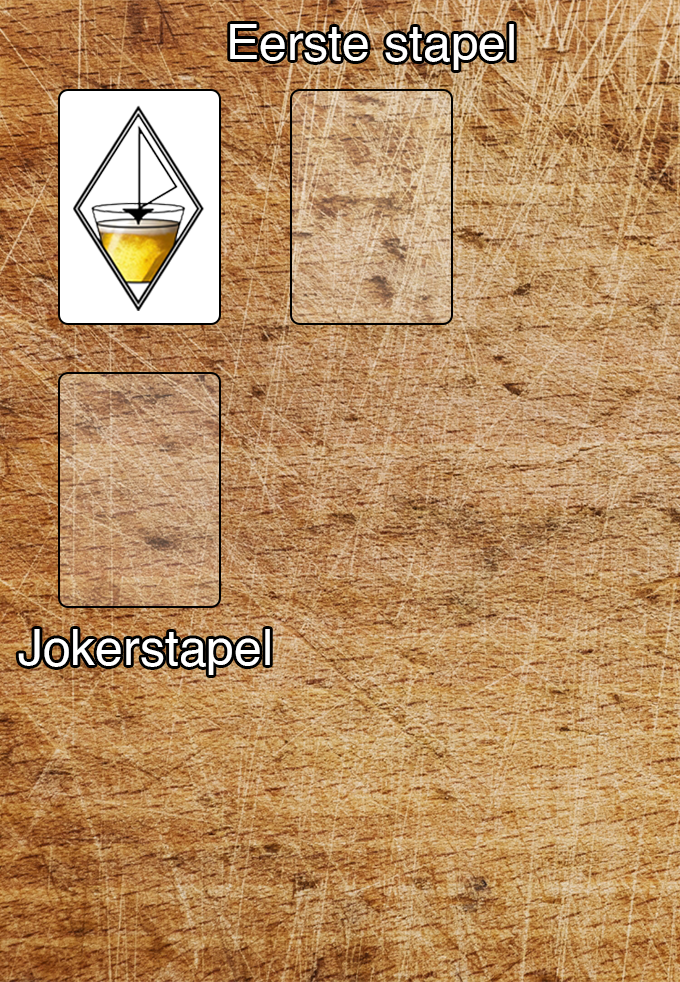
\includegraphics[width=.96\textwidth]{img/Frits_plank_v3.png}
\end{minipage}
\hfill \vrule \hspace{0.3cm}
\begin{minipage}[t]{.48\textwidth}
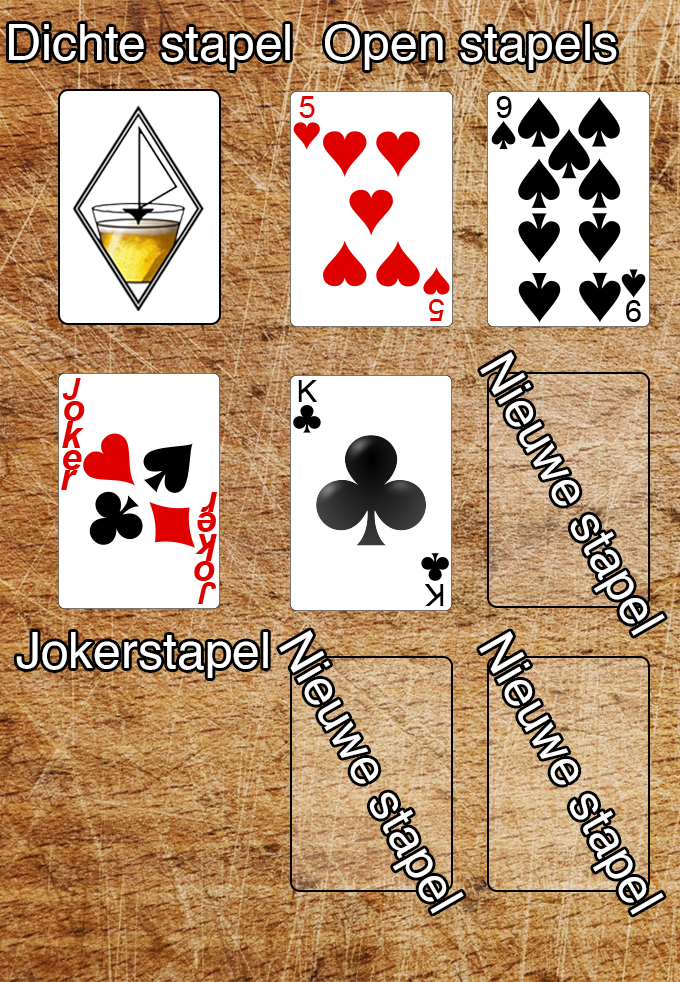
\includegraphics[width=.96\textwidth]{img/Frits_plank_v4_1.png}
\end{minipage}

\vspace{+0.4cm}

\centerline{\Large{\textbf{De volgende pagina beschrijft de zetten}}}
\newpage
\drawBar{Introductie - Vervolg}
\vspace*{0.2cm}
\deelhoofdstuk{Zetten - Andere spelers drinken \ul{niet}}
\noindent
\begin{minipage}[t]{.48\textwidth}
  \zetKortKort{0.40}{1}{Een kaart op een \ul{lagere} kaart van \ul{hetzelfde} symbool leggen.}
  \zetKort{0.40}{2}{Een kaart op een kaart \\\ul{\'e\'en} hoger van \ul{hetzelfde} symbool leggen}{Proost op \quotes{offer Frits} en \textbf{neem een Fritsje}.}
\end{minipage}% This must go next to `\end{minipage}`
\hfill \vrule \hfill
\begin{minipage}[t]{.48\textwidth}
  \zetKortKort{0.40}{3}{Een \kaart{2} op een \kaart{aas} van \newline \ul{hetzelfde} symbool leggen.}
  \zetKortKort{0.40}{4}{Een \kaart{9} op een kaart ongelijk aan een \kaart{joker} leggen.}
\end{minipage}

\deelhoofdstuk{Zet - Kaarten inwisselen}
\noindent

\zetLang{0.20}{5}{Een \kaart{6} op een \kaart{vrouw} leggen}{Leg je kaarten \ul{dicht} op de snijplank, proost op \quotes{Baudet} en \textbf{neem een dubbele Frits}. \Frits legt de kaarten onderop de dichte stapel en geeft je evenveel nieuwe kaarten.}{\ul{\texttt{LET OP}}: Niet uitgaan met deze zet!}

\deelhoofdstuk{Zetten - Andere spelers drinken}
\label{sec:regels_kort}

\noindent
\begin{minipage}[t]{.48\textwidth}
 \zetKort{0.40}{7}{Een \kaart{koning} op een \kaart{harten aas} leggen of andersom}{Andere spelers proosten op \quotes{kut Lisa} en \\\textbf{Fritsen}.}
\end{minipage}
\hfill \vrule \hfill
\begin{minipage}[t]{.48\textwidth}
\zetKort{0.40}{6}{Een \kaart{rode vrouw} op een \kaart{klaveren boer} leggen of andersom}{Andere spelers proosten op \quotes{Chantal} en \\\textbf{Fritsen}.}
\end{minipage}

\vspace{+0.5cm}

\zetLang{0.20}{9}{Een \kaart{vrouw} op een \kaart{vrouw} leggen}{Andere spelers proosten op \quotes{kut Kim} en \textbf{Fritsen}.}{\ul{\texttt{LET OP}}: Als de \kaart{vrouw} op een stapel met drie achtereenvolgende \kaart{vrouwen} wordt gelegd, moeten de andere spelers \textbf{een dubbele Frits nemen}.}

\zetLang{0.20}{8}{Een \kaart{9} op een \kaart{9} leggen}{Andere spelers proosten op \quotes{iedereen dubbel Frits} en \textbf{nemen een dubbele Frits}.}{}

\zetLang{0.20}{10}{Een \kaart{joker} op de jokerstapel leggen}{Begin een nieuwe jokerstapel als er nog geen jokerstapel ligt.}{\ul{\texttt{LET OP}}: Er is maar \ul{\'e\'en} jokerstapel!\\ \ul{\texttt{LET OP}}: Niet uitgaan met deze zet!}

\vspace{+0.4cm}

\centerline{\Large{\textbf{De rest van dit document bevat de volledige spelregels}}}
\newpage
\drawBar{}

\section*{1. Definities}

\beginABCLijst{1}
\item Een acties of belangrijk begrip wordt \textbf{vetgedrukt} weergegeven.

\item Een kaart wordt \ul{\textbf{vetgedrukt en onderstreept}} weergegeven.

\item Een persoon wordt \textbf{[vetgedrukt en tussen vierkante haken]} weergegeven.

\item Een uitspraak of proost wordt \quotes{cursief en tussen aanhalingstekens} weergegeven 

\item Een \textbf{stapel} is één of meer op elkaar gelegde kaarten.

\item De vier typen kaartspelsymbolen of \textbf{symbolen} zijn \ul{\textbf{harten}}, \ul{\textbf{klaveren}}, \ul{\textbf{ruiten}} en \ul{\textbf{schoppen}}. 

\item \label{def:fritsen} \textbf{Fritsen} of \textbf{een Fritsje nemen} is het drinken van minimaal 3 cl bier van minimaal 4 procent alcohol uit een shotglaasje of het drinken van een equivalente hoeveelheid alcohol uit een ander glas.

\item \label{item:enkel_fritsen_equivalent}\textbf{Een Fritsje des nemen}, \textbf{een uittreefritsje nemen}, \textbf{een Lisaatje nemen}, \textbf{een Kimmetje nemen}, \textbf{een Jorisje nemen} zijn equivalent aan \textbf{Fritsen} en \textbf{een Fritsje nemen}. 

\item \label{item:dubbelfritsen_equivalent} \textbf{Dubbelfritsen} en \textbf{een dubbele Frits nemen} zijn equivalent aan twee keer \textbf{Fritsen}.

\item \textbf{Een dubbele Kim nemen}, \textbf{een Erikje nemen} en \textbf{een Thierry'tje nemen} zijn equivalent aan \textbf{dubbelfritsen} en \textbf{een dubbele Frits nemen}.

\item \textbf{[Alle spelers]} zijn diegenen die momenteel aan het Fritsen zijn.

\item \textbf{[Een speler]} is één van \textbf{[alle spelers]}. 

\item De \huidigeSpeler is diegene die momenteel aan de beurt\footnotemark[1] is.  

\item Een \andereSpeler of de \andereSpelers zijn diegene(n) die momenteel \ul{niet} aan de beurt\footnotemark[1] zijn. 

\item De \volgendeSpeler van \eenSpeler is diegene die na hem/haar aan de beurt\footnotemark[1] is. 

\item De \medeSpelers van \eenSpeler zijn \alleSpelers behalve hem/haar.

\item \textbf{[Frits]} is diegene die het meest op \textit{Frits Kastelein}\footnotemark[2] lijkt volgens meer dan de helft van \textbf{[alle spelers]\footnotemark[3]}.

\item \textbf{[Willem]} is diegene die het meest op \textit{Willem Vaandrager}\footnotemark[2] lijkt volgens meer dan de helft van \textbf{[alle spelers]\footnotemark[3]}.

\item \label{item:kim}\textbf{[Kim]} is \textit{Kim de Boer}.

\item \label{item:lisa}\textbf{[Lisa]} is \textit{Lisa de Haan}.

\item \label{item:uitfritsen} \textbf{Uitfritsen} is het neerleggen van de laatste kaart(en) van \textbf{[een speler]}.

\item  \label{item:uitfritsgarantie} \textbf{Uitfritsgarantie} hebben is het niet meer nieuwe kaarten hoeven te pakken en elke beurt\footnotemark[1] kaart(en) kunnen wegleggen.

\item \label{item:uitklaver} \textbf{Uitklaveren} is het \textbf{uitfritsen} met een \kaart{klaveren 3}\footnotemark[4].

\item \label{item:kaarten} \'E\'en \textbf{pak kaarten} bestaat uit: 
    \puntLijst{}
        \item de unieke set kaarten met \textbf{symbolen} schoppen, harten klaveren en ruiten met namen \kaart{2}, \kaart{3}, \kaart{4}, \kaart{5}, \kaart{6}, \kaart{7}, \kaart{8}, \kaart{9}, \kaart{10}, \kaart{boer}, \kaart{vrouw}, \kaart{koning} en \kaart{aas}.
        \item twee jokers en, indien aanwezig, een bridge-kaart.
    \eindPuntLijst{}

\item \label{item:kaarten_2} De waarde van de kaarten in oplopende volgorde zijn \kaart{2}, \kaart{3}, \kaart{4}, \kaart{5}, \kaart{6}, \kaart{7}, \kaart{8}, \kaart{9}, \kaart{10}, \kaart{boer}, \kaart{vrouw}, \kaart{koning} en \kaart{aas}. De rest van de kaarten zijn \kaart{jokers}.

\item \textbf{Dichtfritsen} is een \textbf{stapel} compleet dichtleggen, d.w.z., op die \textbf{stapel} kan alleen nog maar een \ul{\textbf{9}} of een \ul{\textbf{harten aas}} worden gelegd.



\item \label{item:kanonskogel} Een \textbf{kanonskogel} is een shotglaasje van minimaal 3 cl met 50 procent Sambuca en 50 procent Goldstrike met, mits aanwezig, drie druppels tabasco.

\eindABCLijst

\footnotetext[1]{zie het stroomdiagram op de achterkant van dit document}
\footnotetext[2]{zie de foto's op de achterkant van dit document}
\footnotetext[3]{gebruik bij twijfel regel \ref{item:beslissingCriteria}}
\footnotetext[4]{zie regels \ref{zet:Jesse}, \ref{zet:Jesse_2} en \ref{zet:Erik}}
\newpage
\drawBar{}

\hoofdstuk{2}{Regels}

\begin{tabular}{ll}
    \large{$\rightarrow$ Algemeen} & \hspace{0.5cm} \large{pagina \pageref{sec:algemeen_start} t/m \pageref{sec:algemeen_einde}} \\
    \large{$\rightarrow$ Beginfase} van het Spel & \hspace{0.5cm} \large{pagina \pageref{sec:beginfase_start} t/m \pageref{sec:beginfase_einde}}\\
    \large{$\rightarrow$ Vuil Fritsen} & \hspace{0.5cm} \large{pagina \pageref{sec:vuil_fritsen}}\\
    \large{$\rightarrow$ Beurten en Zetten} & \hspace{0.5cm} \large{pagina \pageref{sec:beurten_en_zetten_start} t/m \pageref{sec:beurten_en_zetten_einde}} \\
    \large{$\rightarrow$ Jokers} & \hspace{0.5cm} \large{pagina \pageref{sec:jokers}}\\
    \large{$\rightarrow$ Thierry Baudet en Jesse Klaver} & \hspace{0.5cm} \large{pagina \pageref{sec:thierry}}
\end{tabular}

\deelhoofdstuk{Regels - Algemeen}
\label{sec:algemeen_start}
\beginLijst{2}
    \item Als \eenSpeler \'e\'en van de regels in dit document overtreedt, moet hij/zij:
    \puntLijst{}
        \item Proosten op \quotes{Frits} en \textbf{een Fritsje des nemen}\footnotemark[1].
    \eindPuntLijst{}
\eindLijst{}  

\vervolgLijst{}
    \item Als \eenSpeler het verboden woord \ul{\texttt{ADTEN}} zegt, moet hij/zij:
    \puntLijst{}
    \item Proosten op \quotes{Frits} en \textbf{een Fritsje des nemen}\footnotemark[1]. 
    \eindPuntLijst{}
\eindLijst{}   

\vervolgLijst{}
    \item Als een regel binnen de huidige situatie onduidelijk is of op meerdere manieren geïnterpreteerd kan worden, moet meer dan de helft van \textbf{[alle spelers]} overeenkomen tot een interpretatie van de desbetreffende regel.
\eindLijst{}

\vervolgLijst{}
    \item \label{item:beslissingCriteria} Als meer dan de helft van \textbf{[alle spelers]} het niet eens kan worden over een fritsgerelateerde kwestie gelden de volgende beslissingscriteria (in volgorde van belangrijkheid):
    \numeriekeLijst{}
        \item De beslissing wordt genomen door de grootste groep van \textbf{[alle spelers]} met dezelfde mening over de gerelateerde kwestie. 
        \item De beslissing wordt, wanneer \Frits dit wil, genomen door \textbf{[Frits]}.
        \item De beslissing wordt, wanneer \Willem dit wil, genomen door \textbf{[Willem]}.
        \item De beslissing wordt genomen door de oudste van \textbf{[alle spelers]}.
    \eindNumeriekeLijst{}
\eindLijst{}

\vervolgLijst{}
    \item Als \eenSpeler volgens meer dan de helft van \textbf{[alle spelers]} een domme of onnodige fritsgerelateerde fout maakt, moet hij/zij:
    \puntLijst{}
        \item Proosten op \quotes{Frits} en \textbf{een Fritsje des nemen}\footnotemark[1].
    \eindPuntLijst{}
\eindLijst{}  

\vervolgLijst{}
    \item Voor elke handeling, gebrek aan een handeling of verkeerde uitspraak mag \eenSpeler maximaal twee keer opgelegd worden om te drinken.
\eindLijst{}   

\vervolgLijst{}
    \item Als meer dan de helft van \textbf{[alle spelers]} goedkeurt dat \eenSpeler niet hoeft te drinken, hoeft hij/zij niet te drinken.
\eindLijst{}   

\vervolgLijst{}
    \item Het meer \textbf{Fritsen} dan nodig wordt niet beloond maar wel gewaardeerd.
\eindLijst{}   

\vervolgLijst{}
    \item Als \eenSpeler niet bezig is met een fritsgerelateerde taak, wordt het gewaardeerd als hij/zij lege shotglaasjes vult met de drank die op dat moment gebruikt wordt om te Fritsen.
\eindLijst{}   

\vervolgLijst{}
    \item Als \eenSpeler proost bij het uitvoeren van een fritsgerelateerde taak, moet hij/zij dit hoor- en verstaanbaar voor minimaal twee derde van \alleSpelers doen.
\eindLijst{} 

\vervolgLijst{}
    \item \EenSpeler hoeft niet de waarheid te spreken als hij/zij zegt dat hij/zij \textbf{uitfritsgarantie}\footnotemark[2] heeft.
\eindLijst{}   

\footnotetext[1]{\textbf{een Fritsje des nemen} is equivalent aan \textbf{Fritsen} (zie definitie \ref{item:enkel_fritsen_equivalent})}
\footnotetext[2]{zie definitie \ref{item:uitfritsgarantie}}

\newpage
\drawBar{Regels - Vervolg}
\deelhoofdstuk{Regels - Algemeen - Vervolg}

\customBoxItalic{Je kunt gewoon naar het toilet en bevorderende fritsgerelateerde handeling uitvoeren. Voor deze gevallen kan het spel worden gepauzeerd: Niemand mag dan een zet doen.}

\vervolgLijst{}
    \item Als \eenSpeler aangeeft dat hij/zij naar het toilet wilt, wordt het spel stilgelegd totdat hij/zij terug van het toilet is.
    \label{regel:stilleggen_1}
\eindLijst{}   

\vervolgLijst{}
    \item Als \eenSpeler een handeling wilt uitvoeren die het huidige potje Fritsen bevordert die door meer dan de helft van \textbf{[alle spelers]} wordt goedgekeurd, mag het spel stilgelegd worden totdat hij/zij de desbetreffende handeling heeft uitgevoerd.
    \label{regel:stilleggen_2}
\eindLijst{}  

\customBoxItalic{Pak alléén kaarten van de dichte stapel en géén kaarten van de open stapels.}

\vervolgLijst{}
    \item Als \eenSpeler in de \ul{dichte} \textbf{stapel} kijkt, moet hij/zij:
    \puntLijst{}
        \item Proosten op \quotes{vierdubbel Frits} en \ul{twee keer} \textbf{een dubbele Frits nemen}[REFERENTIE]. 
        \item De \ul{dichte} \textbf{stapel} goed en zichtbaar schudden volgens meer dan de helft van \\ \textbf{[alle spelers]}.
        \item Twee \ul{dichte} kaarten pakken van bovenop de \ul{dichte} \textbf{stapel}.
    \eindPuntLijst{}
    \label{regel:kijken_in_dichte_stapel}
\eindLijst{}  

\vervolgLijst{}
    \item Als \eenSpeler één kaart of meerdere kaarten van één van de \ul{open} \textbf{stapels} pakt en niet regel \ref{regel:kaarten_terugnemen_1}, \ref{regel:kaarten_terugnemen_2}, \ref{regel:kaarten_terugnemen_3} of \ref{regel:kaarten_terugnemen_4} aan het toepassen is, moet hij/zij:
    \puntLijst{}
       \item Proosten op \quotes{Frits} en \textbf{een Fritsje des nemen}\footnotemark[3].
        \item De net gepakte kaart(en) in dezelfde volgorde \ul{open} terugleggen op de desbetreffende \ul{open} \textbf{stapel}.
    \eindPuntLijst{}
\eindLijst{}  

\customBoxItalic{Ga zorgvuldig om met de shotglaasjes, regelboekjes en speelkaarten.}

\vervolgLijst{}
    \item \EenSpeler mag niet een shotglaasje omgooien.
\eindLijst{} 

\vervolgLijst{}
    \item \EenSpeler mag niet een fritsgerelateerde document natmaken.
\eindLijst{} 

\vervolgLijst{}
    \item \EenSpeler mag op fritsgerelateerde documenten alleen fritsgerelateerde zaken schrijven.
\eindLijst{}

\vervolgLijst{}
    \item \EenSpeler mag geen kaarten natmaken die bij het huidige potje Fritsen gebruikt worden.
\eindLijst{}  

\vervolgLijst{}
    \item \EenSpeler mag niet zijn/haar kaarten of een deel hiervan op de grond laten vallen.
\eindLijst{}  

\footnotetext[1]{\textbf{een Fritsje des nemen} is equivalent aan \textbf{Fritsen} (zie definitie \ref{item:enkel_fritsen_equivalent})}

\newpage
\drawBar{Regels - Vervolg}
\deelhoofdstuk{Regels - Algemeen - Vervolg}
\label{sec:algemeen_einde}

\customBoxItalic{Laat niemand in je kaarten kijken en, wanneer gevraagd, vertel hoeveel je er hebt.}

\vervolgLijst{}
    \item \EenSpeler mag te allen tijde in de kaarten van \alleSpelers kijken.
\eindLijst{}

\vervolgLijst{}
    \item \EenSpeler mag niet de kaarten aanraken van zijn/haar \medeSpelers die bezig is met een fritsgerelateerde taak of die door hem/haar vastgehouden worden.
\eindLijst{}  

\vervolgLijst{}
    \item Als \eenSpeler kaarten vast heeft van zijn/haar \medeSpelers, moet hij/zij deze binnen 9 seconden teruggeven.
\eindLijst{}

\vervolgLijst{}
    \item \EenSpeler is verplicht naar waarheid te vertellen hoeveel kaarten hij/zij in zijn/haar handen heeft wanneer dit gevraagd wordt door zijn/haar \textbf{[medespelers]}.
\eindLijst{}   

\customBoxItalic{Het is belangrijk dat je serieus meespeelt. Zo niet, dan moet je stoppen met spelen.}

\vervolgLijst{}
    \item Als \eenSpeler volgens minimaal twee derde van \alleSpelers niet serieus meedoet met het huidige potje Fritsen, worden de volgende handelingen in de gegeven volgorde uitgevoerd:
    \numeriekeLijst{}
        \item Één van de volgende acties:
        \puntLijst{}
            \item Zijn/haar kaarten worden onder de \ul{dichte} \textbf{stapel} gelegd als er een \ul{dichte} \textbf{stapel} is. 
            \item Zijn/haar kaarten worden als nieuwe \ul{dicht}e \textbf{stapel} neergelegd als er geen bestaande \ul{dichte} \textbf{stapel} is. 
        \eindPuntLijst{}
        \item De desbetreffende speler stopt met Fritsen.
    \eindNumeriekeLijst{}
\eindLijst{}

\vervolgLijst{}
    \item Als \eenSpeler volgens minimaal twee derde van \alleSpelers niet serieus meedoet met het huidige potje Fritsen, mogen \\ \alleSpelers te allen tijde zijn/haar kaarten pakken.
\eindLijst{}

\footnotetext[2]{zie pagina \pageref{sec:introductie}}
\footnotetext[3]{\textbf{een Fritsje des nemen} is equivalent aan \textbf{Fritsen} (zie definitie \ref{item:enkel_fritsen_equivalent})}

\newpage
\drawBar{Regels - Vervolg}
\deelhoofdstuk{Regels - Beginfase van het Spel}
\label{sec:beginfase_start}

\customBoxItalic{Fritsen begint nadat \Frits en \Willem zijn bepaald. Hierna schudt iemand de kaarten en geeft \Frits iedereen vijf \ul{dichte} startkaarten om vervolgens de eerste stapel open te leggen. Je hebt nu de mogelijkheid om te \textbf{vuil Fritsen}. De regels in deze sectie beschrijven het spelverloop op pagina \pageref{sec:introductie}.}

\vervolgLijst{}
    \item Fritsen wordt met minimaal 2 en maximaal 10 personen gespeeld.
\eindLijst{}

\vervolgLijst{}
    \item Fritsen is begonnen zodra \Frits en \Willem zijn bepaald.
    \label{regel:Willen_Frits_bepalen}
\eindLijst{}

\vervolgLijst{}
    \item \Frits moet, nadat regel \ref{regel:Willen_Frits_bepalen} is toegepast, binnen 99 seconden ervoor zorgen dat één van \alleSpelers kan \textbf{vuil Fritsen}.
\eindLijst{}

\customBoxItalic{Fritsen wordt met één of twee pakken kaarten gespeeld. De kaarten moeten goed en zichtbaar worden geschud. Het wordt gewaardeerd wanneer \Frits de kaarten schudt, echter kan \Frits iemand verplichten om te schudden.}

\vervolgLijst{}
    \item Fritsen wordt, tenzij anders aangegeven, tot en met 6 spelers met één \textbf{pak kaarten}\footnotemark[1] en tussen de 7 en 10 personen met twee \textbf{pakken kaarten}\footnotemark[1] gespeeld.
\eindLijst{}

\vervolgLijst{}
    \item Fritsen wordt met twee \textbf{pakken kaarten}\footnotemark[1] gespeeld wanneer de groep van \alleSpelers minder dan 7 spelers bevat en meer dan de helft van \alleSpelers dit goedkeuren. 
\eindLijst{}

\vervolgLijst{}
    \item Het \textbf{pak kaarten}\footnotemark[1] dat of de \textbf{pakken kaarten}\footnotemark[1] die gebruikt worden voor het huidige potje Fritsen moeten goed volgens en zichtbaar voor meer dan de helft van \alleSpelers geschud worden.
    \label{regel:goed_zichtbaar_schudden}
\eindLijst{}

\vervolgLijst{}
    \item Als \eenSpeler regel \ref{regel:goed_zichtbaar_schudden} niet naleeft, moet hij/zij:
    \puntLijst{}
        \item Proosten op \quotes{Frits} en \textbf{een Fritsje des nemen}\footnotemark[2].
        \item Alle kaarten verzamelen en schudden volgens regel \ref{regel:goed_zichtbaar_schudden}.
        \item Alle kaarten aan \Frits geven zodat hij/zij ze kan delen.
    \eindPuntLijst{}
\eindLijst{}

\vervolgLijst{}
    \item \Frits kan \eenSpeler verplichten om de kaarten te schudden volgens regel \ref{regel:goed_zichtbaar_schudden} door:
    \puntLijst{}
        \item Dit aan te geven en \textbf{een dubbele Frits}\footnotemark[3] te nemen.
    \eindPuntLijst{}
\eindLijst{}

\customBoxItalic{Onderstaande regels beschrijven stap 2 van het spelverloop op pagina \pageref{sec:introductie}.}

\vervolgLijst{}
    \item \Willem moet, voordat \Frits begonnen is met delen, links plaatsnemen van \textbf{[Frits]}.
    \label{regel:Willen_links_van_Frits}
\eindLijst{}

\vervolgLijst{}
    \item Als \Frits en \Willem regel \ref{regel:Willen_links_van_Frits} niet naleven, moeten zij:
    \puntLijst{}
        \item Proosten op \quotes{Frits} en \textbf{een Fritsje des nemen}\footnotemark[1].
        \item Zich positioneren volgens regel \ref{regel:Willen_links_van_Frits}.
    \eindPuntLijst{}
\eindLijst{}

\footnotetext[1]{zie definities \ref{item:kaarten} en \ref{item:kaarten_2}}
\footnotetext[2]{\textbf{een Fritsje des nemen} is equivalent aan \textbf{Fritsen} (zie definitie \ref{item:enkel_fritsen_equivalent})}
\footnotetext[3]{\textbf{een dubbele Frits nemen} is equivalent aan twee keer \textbf{Fritsen} (zie definities \ref{item:enkel_fritsen_equivalent} en \ref{item:dubbelfritsen_equivalent})}

\newpage
\drawBar{Regels - Vervolg}
\deelhoofdstuk{Regels - Beginfase van het spel - Vervolg}
\label{sec:beginfase_einde}

\customBoxItalic{Onderstaande regels beschrijven stap 3 en 4 van het spelverloop op pagina \pageref{sec:introductie}.}

\vervolgLijst{}
    \item Alleen \Frits mag delen\footnotemark[1].
    \label{regel:delen_Frits}
\eindLijst{}

\vervolgLijst{}
    \item \Frits is niet verplicht om tijdens het delen\footnotemark[1] de kaarten netjes, recht of gepast te positioneren volgens meer dan de helft van \textbf{[alle spelers]}.
\eindLijst{}

\vervolgLijst{}
    \item Als \Frits deelt\footnotemark[1], moet hij/zij \alleSpelers vijf \ul{dichte} kaarten geven van de \ul{dichte} \textbf{stapel} door deze één voor één van bovenop de \ul{dichte} \textbf{stapel} te pakken.
    \label{regel:delen_Frits_5_kaarten_1}
\eindLijst{}

\vervolgLijst{}
    \item Als \Frits deelt\footnotemark[1], moet hij/zij \alleSpelers om de beurt één \ul{dichte} kaart geven.
    \label{regel:delen_Frits_5_kaarten_2}
\eindLijst{}

\vervolgLijst{}
    \item Nadat \Frits regels \ref{regel:delen_Frits_5_kaarten_1} en \ref{regel:delen_Frits_5_kaarten_2} heeft toegepast, moet hij/zij direct de \ul{bovenste} kaart van de \ul{dichte} \textbf{stapel} openleggen direct naast de \ul{dichte} \textbf{stapel}.
    \label{regel:eerst_kaart_open}
\eindLijst{}   

\vervolgLijst{}
    \item Als \Frits een \kaart{joker}\footnotemark[2] openlegt in regel \ref{regel:eerst_kaart_open}, moet hij/zij nogmaals de \ul{bovenste} kaart van de \ul{dichte} \textbf{stapel} \ul{open} op de enige \ul{open} \textbf{stapel} leggen totdat deze geen \kaart{joker}\footnotemark[2] is.
    \label{regel:eerste_kaart_open_joker}
\eindLijst{}   

\vervolgLijst{}
    \item \EenSpeler mag alleen zijn/haar eigen \textbf{stapel} met \ul{dichte} kaarten pakken nadat \Frits gedeeld\footnotemark[1] heeft.
   \label{regel:andere_kaarten_pakken}
\eindLijst{}

\vervolgLijst{}
    \item Als \eenSpeler regel \ref{regel:delen_Frits}, \ref{regel:delen_Frits_5_kaarten_1}, \ref{regel:delen_Frits_5_kaarten_2}, \ref{regel:eerst_kaart_open}, \ref{regel:eerste_kaart_open_joker} of \ref{regel:andere_kaarten_pakken} niet naleeft, moet hij/zij:
    \puntLijst{}
        \item Proosten op \quotes{Frits} en \textbf{een Fritsje des nemen}\footnotemark[3].
        \item Alle kaarten verzamelen en schudden volgens regel \ref{regel:goed_zichtbaar_schudden}.
        \item Alle kaarten aan \Frits geven zodat hij/zij ze kan delen.
    \eindPuntLijst{}
\eindLijst{}

\vervolgLijst{}
    \item Als \eenSpeler kaarten in zijn/haar hand neemt terwijl \Frits deelt\footnotemark[1], moet hij/zij:
     \puntLijst{}
         \item Proosten op \quotes{Frits} en \textbf{een Fritsje des nemen}\footnotemark[3].
         \item Zijn/haar gepakte kaart(en) in zijn/haar hand houden.
     \eindPuntLijst{}
\eindLijst{}

\customBoxItalic{Onderstaande regels beschrijven stap 6 van het spelverloop op pagina \pageref{sec:introductie}.}

\vervolgLijst{}
    \item Tijdens het Fritsen, nadat \Willem zijn/haar eerste kaart(en) heeft opgelegd, zijn\\ \alleSpelers in de richting van de klok aan de beurt\footnotemark[4].
\eindLijst{}


\footnotetext[1]{zie \texttt{stap 3} op pagina \pageref{sec:introductie}}
\footnotetext[2]{zie definitie \ref{item:kaarten}}
\footnotetext[3]{\textbf{een Fritsje des nemen} is equivalent aan \textbf{Fritsen} (zie definitie \ref{item:enkel_fritsen_equivalent})}
\footnotetext[4]{zie het stroomdiagram op de achterkant van dit document}

\newpage
\drawBar{Regels - Vervolg}
\deelhoofdstuk{Regels - Vuil Fritsen}
\label{sec:vuil_fritsen}

\customBoxItalic{\textbf{Vuil Fritsen} is het drinken en daarna inwisselen van je vijf startkaarten voordat \Willem als \ul{eerste} aan de beurt\footnotemark[1] is. Een slechte hand bestaat uit meerdere kaarten met de waarde lager dan een \ul{\textbf{9}}. Je mag zo vaak \textbf{vuil Fritsen} als je wilt.}

\vervolgLijst{}
    \item Als \eenSpeler aan het \textbf{vuil Fritsen} is, moet hij/zij alle volgende acties in de gegeven volgorde uitvoeren:
    \puntLijst{}
        \item Proosten op \quotes{vuile Frits} en \textbf{een dubbele Frits nemen}\footnotemark[2].
        \item Zijn/haar kaarten \ul{dicht} op de tafel leggen.
        \item Vijf nieuwe \ul{dichte} kaarten van \Frits in ontvangst nemen van bovenop de \ul{dichte} \textbf{stapel} nadat \Frits de \ul{oude} kaarten \ul{dicht} onderop de \ul{dichte} \textbf{stapel} gelegd heeft.
    \eindPuntLijst{}
     \label{regel:zet_vuil_fritsen}
\eindLijst{}

\vervolgLijst{}
    \item Als minimaal twee derde van \alleSpelers bepaalt dat, voordat regel \ref{regel:zet_vuil_fritsen} toegepast is, géén van \alleSpelers mag \textbf{vuil Fritsen}, mag géén van \alleSpelers \textbf{vuil Fritsen}.
    \label{regel:skip_vuil_fritsen}
\eindLijst{}

\vervolgLijst{}
    \item Als \eenSpeler ongelijk aan \Frits kaarten van de \ul{dichte} \textbf{stapel} pakt tijdens het uitvoeren van zet \ref{regel:zet_vuil_fritsen}, moet hij/zij:
    \puntLijst{}
        \item Proosten op \quotes{Frits} en \textbf{een Fritsje des nemen}\footnotemark[3].
        \item Zijn/haar gepakte kaart(en) in zijn/haar hand houden.
    \eindPuntLijst{}
\eindLijst{}

\vervolgLijst{}
    \item \EenSpeler mag alleen \textbf{vuil Fritsen} als \ul{g\'e\'en} van \textbf{[alle spelers]} aan de beurt\footnotemark[1] geweest is en regel \ref{regel:skip_vuil_fritsen} niet is toegepast. 
\eindLijst{}

\vervolgLijst{}
    \item \EenSpeler mag, als regel \ref{regel:skip_vuil_fritsen} niet is toegepast, zo vaak \textbf{vuil Fritsen} als hij/zij wilt. 
\eindLijst{}

\vervolgLijst{}
    \item \EenSpeler mag alleen proosten op \quotes{vuile Frits} als hij/zij aan het \textbf{vuil Fritsen} is.
\eindLijst{}

\vervolgLijst{}
    \item Bij \textbf{vuil Fritsen} geldt wie het eerst komt, het eerst maalt.
\eindLijst{}

\customBoxItalic{Je hebt genoeg tijd om te beslissen of je wilt \textbf{vuil Fritsen}.}

\vervolgLijst{}
    \item \Willem mag de eerste 99 seconden na het uitdelen van de kaarten alleen met zijn/haar beurt beginnen wanneer \textbf{[alle spelers]} dit goedkeuren of regel \ref{regel:skip_vuil_fritsen} toegepast is. 
    \label{regel:vuile_frits_1}
\eindLijst{}

\vervolgLijst{}
    \item \Willem mag pas na 99 seconden na de laatste \textbf{vuile Frits} met zijn/haar beurt beginnen of wanneer \textbf{[alle spelers]} het goedkeuren dat hij/zij eerder begint.
    \label{regel:vuile_frits_2}
\eindLijst{}

\vervolgLijst{}
    \item Als \Willem regel \ref{regel:vuile_frits_1} of \ref{regel:vuile_frits_2} niet naleeft, moet hij/zij:
    \puntLijst{}
        \item Proosten op \quotes{Frits} en \textbf{een Fritsje des nemen}\footnotemark[3].
        \item Zijn/haar beurt\footnotemark[1] meteen beëindigen.
        \item Zijn/haar opgelegde kaart(en) terug in zijn/haar hand nemen.
    \eindPuntLijst{}
    \label{regel:kaarten_terugnemen_1}
\eindLijst{}

\footnotetext[1]{zie het stroomdiagram op de achterkant van dit document}
\footnotetext[2]{\textbf{een dubbele Frits nemen} is equivalent aan twee keer \textbf{Fritsen} (zie definities \ref{item:enkel_fritsen_equivalent} en \ref{item:dubbelfritsen_equivalent})}
\footnotetext[3]{\textbf{een Fritsje des nemen} is equivalent aan \textbf{Fritsen} (zie definitie \ref{item:enkel_fritsen_equivalent})}

\newpage
\drawBar{Regels - Vervolg}
\deelhoofdstuk{Regels - Beurten en Zetten}
\label{sec:beurten_en_zetten_start}

\customBoxItalic{Met Fritsen is iedereen met de klok mee aan de beurt. Zolang je nog kaarten hebt, leg je elke beurt \'e\'en of meer kaarten weg en bestaat de mogelijkheid dat je twee nieuwe kaarten moet pakken. Het stroomdiagram op achterkant van dit document beschrijft hoe een beurt verloopt. Pagina \pageref{sec:regels_kort}, en hoofdstuk 6 in detail, bevatten een overzicht van de mogelijke zetten en de bijbehorende acties die moeten worden uitgevoerd.}

\vervolgLijst{}
    \item Als \eenSpeler langer dan 99 seconden over zijn/haar beurt\footnotemark[1] doet, moet hij/zij:
    \puntLijst{}
        \item Proosten op \quotes{Frits} en \textbf{een Fritsje des nemen}\footnotemark[2]
        \item Twee \ul{dichte} kaarten pakken van bovenop de \ul{dichte} \textbf{stapel} wanneer hij/zij dit nog niet gedaan heeft in zijn/haar beurt.
        \item Zijn/haar beurt\footnotemark[1] meteen beëindigen.
    \eindPuntLijst{}
    \label{regel:beurt_langer_dan_99}
\eindLijst{}

\customBoxItalic{Onderstaand regels beschrijven het stroomdiagram op de achterkant van dit document.}

\vervolgLijst{}
    \item \EenSpeler mag meteen na het beginnen van zijn/haar beurt\footnotemark[1] \'e\'en zet\footnotemark[3] doen.
\eindLijst{}

\vervolgLijst{}
    \item \label{regel:twee_kaarten} Als de \huidigeSpeler geen zet\footnotemark[3] doet voordat hij/zij twee nieuwe \ul{dichte} kaarten heeft gepakt, moet hij/zij:
    \puntLijst{}
        \item \textbf{Fritsen} en daarna twee nieuwe \ul{dichte} kaarten pakken van bovenop de \ul{dichte} \textbf{stapel}.
        \item Één van de volgende acties uitvoeren:
        \numeriekeLijst{}
            \item Een zet\footnotemark[3] doen.
            \item Een nieuwe \ul{open} \textbf{stapel} beginnen.
        \eindNumeriekeLijst{}
     \eindPuntLijst{}
\eindLijst{}

\vervolgLijst{}
    \item Proosten op \quotes{Frits} tijdens het uitvoeren van regel \ref{regel:twee_kaarten} is niet verplicht maar wordt wel gewaardeerd.
\eindLijst{}

\vervolgLijst{}
    \item Als \eenSpeler twee \ul{dichte} kaarten moet pakken tijdens het uitvoeren van regel \ref{regel:kijken_in_dichte_stapel}, \ref{regel:beurt_langer_dan_99} of \ref{regel:twee_kaarten} terwijl er g\'e\'en \ul{dichte} kaarten meer zijn, hoeft hij/zij geen \ul{dichte} kaarten te pakken.
    \label{item:geen_kaart_1}
\eindLijst{}

\vervolgLijst{}
    \item Als \eenSpeler twee \ul{dichte} kaarten moet pakken tijdens het uitvoeren van regel \ref{regel:kijken_in_dichte_stapel}, \ref{regel:beurt_langer_dan_99} of \ref{regel:twee_kaarten} terwijl er nog maar \'e\'en \ul{dichte} kaart is, moet hij/zij \'e\'en \ul{dichte} kaart pakken.
    \label{item:geen_kaart_2}
\eindLijst{}

\vervolgLijst{}
    \item Als \eenSpeler méér kaart(en) dan nodig pakt van de \ul{dichte} \textbf{stapel}, moet hij/zij deze in zijn/haar hand houden.
\eindLijst{}

\vervolgLijst{}
    \item \EenSpeler is niet verplicht om een zet\footnotemark[3] te doen voordat en nadat hij/zij twee nieuwe kaarten heeft gepakt.
\eindLijst{}

\vervolgLijst{}
    \item \EenSpeler moet in zijn/haar beurt\footnotemark[1] \'e\'en zet\footnotemark[3] doen of \'e\'en nieuwe \ul{open} \textbf{stapel} beginnen als hij/zij nog kaarten in zijn/haar hand heeft.
\eindLijst{}

\footnotetext[1]{zie het stroomdiagram op de achterkant van dit document}
\footnotetext[2]{\textbf{een Fritsje des nemen} is equivalent aan \textbf{Fritsen} (zie definitie \ref{item:enkel_fritsen_equivalent})}
\footnotetext[3]{zie pagina \pageref{sec:regels_kort}, \pageref{sec:zettenLang} en \pageref{sec:zettenLang_2}}

\newpage
\drawBar{Regels - Vervolg}
\deelhoofdstuk{Regels - Beurten en Zetten - Vervolg}

\customBoxItalic{Leg je kaarten netjes neer.}

\vervolgLijst{}
    \item Als \eenSpeler een kaart neerlegt, moet hij/zij deze netjes, recht en gepast positioneren volgens meer dan de helft van \textbf{[alle spelers]}.
    \label{regel:kaart_netjes_1}
\eindLijst{}

\vervolgLijst{}
    \item Als \eenSpeler één van de opgelegde kaart(en) of één van de kaarten van de \ul{dichte} \textbf{stapel} verplaatst, moet hij/zij deze netjes, recht en gepast positioneren volgens meer dan de helft van \textbf{[alle spelers]}.
    \label{regel:kaart_netjes_2} 
\eindLijst{}

\vervolgLijst{}
    \item Als \eenSpeler regel \ref{regel:kaart_netjes_1} of \ref{regel:kaart_netjes_2} niet naleeft, moet hij/zij:
    \puntLijst{}
        \item Proosten op \quotes{Frits} en \textbf{een Fritsje des nemen}\footnotemark[1].
        \item Alle \ul{open} \textbf{stapel(s)} en de \ul{dichte} \textbf{stapel} recht, netjes en gepast positioneren volgens meer dan de helft van \textbf{[alle spelers]}. 
    \eindPuntLijst{}
\eindLijst{}

\customBoxItalic{Proost alléén op het juiste moment.}

\vervolgLijst{}
    \item \EenSpeler mag alleen proosten op \quotes{offer Frits}, \quotes{kut Lisa}, \quotes{supermooi Lisa}, \quotes{kut Kim}, \quotes{supermooi Kim} en \quotes{Chantal} als hij/zij de bijbehorende zet aan het uitvoeren is\footnotemark[2]. 
\eindLijst{}

\customBoxItalic{Leg alléén een kaart op wanneer dit mag.}

\vervolgLijst{}
    \item \EenSpeler mag geen kaart(en) opleggen die niet in lijn zijn met de regels en zetten.
    \label{regel:ongeldige_zet}
\eindLijst{}

\vervolgLijst{}
    \item \EenSpeler mag, tenzij elders beschreven, niet voor zijn/haar beurt\footnotemark[3] opleggen.
    \label{regel:voor_beurt_opleggen}
\eindLijst{}

\vervolgLijst{}
    \item \EenSpeler mag geen zet doen wanneer het spel is stilgelegd.
    \label{regel:tijdens_pauze_opleggen}
\eindLijst{}

\vervolgLijst{}
    \item Als \eenSpeler regel \ref{regel:ongeldige_zet}, \ref{regel:voor_beurt_opleggen} of \ref{regel:tijdens_pauze_opleggen} niet naleeft, moet hij/zij:
    \puntLijst{}
        \item De opgelegde kaart(en) terug in zijn/haar hand nemen.
        \item Proosten op \quotes{Frits} en \textbf{een Fritsje des nemen}\footnotemark[1].
    \eindPuntLijst{}
    \label{regel:kaarten_terugnemen_2}
\eindLijst{}

\vervolgLijst{}
    \item Als \eenSpeler één kaart of meerdere kaarten oplegt die niet in lijn zijn met de regels en zetten, heeft deze kaart of hebben deze kaarten geen drinkwaarde.
\eindLijst{}  

\footnotetext[1]{\textbf{een Fritsje des nemen} is equivalent aan \textbf{Fritsen} (zie definitie \ref{item:enkel_fritsen_equivalent})}
\footnotetext[2]{zie zetten \ref{zet:offer_frits}, \ref{zet:lisa} en \ref{zet:kim} op pagina \pageref{zet:kim} en zet \ref{zet:joris} op pagina \pageref{zet:joris}}
\footnotetext[3]{zie het stroomdiagram op de achterkant van dit document}

\newpage
\drawBar{Regels - Vervolg}
\deelhoofdstuk{Regels - Beurten en Zetten - Vervolg}
\label{sec:beurten_en_zetten_einde}

\customBoxItalic{Blijf goed opletten wie er aan de beurt\footnotemark[1] of geen kaarten meer heeft.}

\vervolgLijst{}
    \item \EenSpeler moet van \alleSpelers weten wie aan de beurt\footnotemark[1] is en wie \textbf{uitgefritst}\footnotemark[2] zijn.
\eindLijst{}

\vervolgLijst{}
    \item Als niemand van \alleSpelers weet of wil vertellen wie aan de beurt\footnotemark[1] is, is \Frits aan de beurt\footnotemark[1].
\eindLijst{}

\vervolgLijst{}
    \item \EenSpeler kan zijn/haar \medeSpelers dwingen om naar waarheid te vertellen wie aan de beurt\footnotemark[1] is door:
    \puntLijst{}
        \item Dit aan te geven en \textbf{een Fritsje te nemen}\footnotemark[3].
    \eindPuntLijst{}
\eindLijst{}

\customBoxItalic{Vergeet niet te proosten op \quotes{laatste Frits} (laatste kaart) en de juiste handelingen uit te voeren wanneer je uitgefritst bent of als laatste nog kaarten in je hand hebt.}

\vervolgLijst{}
    \item Als \eenSpeler na het opleggen nog \'e\'en kaart in zijn/haar hand heeft, moet hij/zij:
    \puntLijst{}
        \item Hoor- en verstaanbaar \quotes{laatste Frits} zeggen voor minimaal twee derde van \\ \textbf{[alle spelers]}.
    \eindPuntLijst{}
    \label{regel:laatste_frits_1}
\eindLijst{}

\vervolgLijst{}
    \item Als de \huidigeSpeler na het opleggen van zijn/haar kaart(en) \textbf{uitgefritst}\footnotemark[4] is, moet hij/zij:
    \puntLijst{}
        \item Proosten op \quotes{Frits} en \textbf{een uittreefritsje nemen}\footnotemark[3].
    \eindPuntLijst{}
    \label{regel:laatste_frits_2}
\eindLijst{}

\vervolgLijst{}
    \item Als \eenSpeler regel \ref{regel:laatste_frits_2} niet naleeft, moet hij/zij:
    \puntLijst{}
        \item Proosten op \quotes{Frits} en \textbf{een Fritsje des nemen}\footnotemark[3].
        \item Proosten op \quotes{Frits} en \textbf{een uittreefritsje nemen}\footnotemark[3].
    \eindPuntLijst{}
\eindLijst{}

\vervolgLijst{}
    \item Als \eenSpeler als laatste van \alleSpelers nog niet \textbf{uitgefritst}\footnotemark[2] is, moet hij/zij:
    \puntLijst{}
        \item Proosten op \quotes{dubbel Frits} en \textbf{een dubbele Frits nemen}\footnotemark[4].
    \eindPuntLijst{}
\eindLijst{}

\customBoxItalic{Onderstaande regels beschrijven wanneer je beurt ten einde is.}

\vervolgLijst{}
    \item Een beurt\footnotemark[1] is voorbij nadat de \huidigeSpeler al zijn/haar beurtgerelateerde taken heeft verricht.
\eindLijst{}

\vervolgLijst{}
    \item De beurt\footnotemark[1] van \eenSpeler is meteen ten einde wanneer hij/zij \textbf{uitgefritst}\footnotemark[2] is aan het begin van zijn/haar beurt. 
\eindLijst{}

\vervolgLijst{}
    \item Als er nog maar \textbf{[\'e\'en speler]} niet \textbf{uitgefritst}\footnotemark[2] is en niemand van \alleSpelers meer hoeft te drinken, is het spel afgelopen.
\eindLijst{}

\vervolgLijst{}
    \item \textbf{[Alle spelers]} moeten blijven meespelen totdat nog maar \textbf{[één speler]} niet \textbf{uitgefritst}\footnotemark[3] is en hij/zij al zijn/haar beurtgerelateerde taken heeft verricht.
\eindLijst{}  

\vervolgLijst{}
    \item \textbf{[Alle spelers]} moeten blijven meespelen totdat niemand van \alleSpelers meer hoeft te drinken.
\eindLijst{} 

\footnotetext[1]{zie het stroomdiagram op de achterkant van dit document}
\footnotetext[2]{\textbf{uitfritsen} is het neerleggen van je laatste kaart(en) (zie definitie \ref{item:uitfritsen})}
\footnotetext[3]{\textbf{een uittreefritsje nemen} en \textbf{een Fritsje des nemen} zijn equivalent aan \textbf{Fritsen} (zie definitie \ref{item:enkel_fritsen_equivalent})}
\footnotetext[4]{\textbf{een dubbele Frits nemen} is equivalent aan twee keer \textbf{Fritsen} (zie definities \ref{item:enkel_fritsen_equivalent} en \ref{item:dubbelfritsen_equivalent})}



\newpage
\drawBar{Regels - Vervolg}
\deelhoofdstuk{Regels - Jokers}
\label{sec:jokers}

\customBoxItalic{Tijdens je beurt\footnotemark[1] kun je andere spelers laten drinken door een \kaart{joker}\footnotemark[2] op te leggen. De \kaart{joker}\footnotemark[2] heeft zijn eigen stapel en uitgaan met een \kaart{joker}\footnotemark[2] is niet toegestaan.}

\vervolgLijst{}
    \item Er moeten 2 of 3 \kaart{jokers}\footnotemark[2] per kaartspel gebruikt worden.
\eindLijst{}

\vervolgLijst{}
    \item \EenSpeler mag niet \textbf{uitfritsen}\footnotemark[4] met een \kaart{joker}\footnotemark[2].
    \label{regel:joker_1}
\eindLijst{}

\vervolgLijst{}
    \item \EenSpeler mag niet een nieuwe \textbf{jokerstapel} beginnen als er al \'e\'en ligt.
    \label{regel:joker_2}
\eindLijst{}

\vervolgLijst{}
    \item \EenSpeler mag, tenzij anders aangegeven, niet een kaart ongelijk aan een \kaart{joker}\footnotemark[2] op de \textbf{jokerstapel} leggen.
    \label{regel:joker_3}
\eindLijst{}

\vervolgLijst{}
    \item Als \eenSpeler een \kaart{joker}\footnotemark[2] neerlegt moet deze zich direct naast de \ul{dichte} \textbf{stapel} bevinden.
    \label{regel:plaats_joker}
\eindLijst{}

\vervolgLijst{}
    \item \EenSpeler mag niet een kaart opleggen waardoor de \textbf{jokerstapel} zich niet direct naast de \ul{dichte} \textbf{stapel} kan bevinden.
    \label{regel:joker_4}
\eindLijst{}

\vervolgLijst{}
    \item Als \eenSpeler regel \ref{regel:joker_1}, \ref{regel:joker_2}, \ref{regel:joker_3}, \ref{regel:plaats_joker} of \ref{regel:joker_4} niet naleeft, moet hij/zij:
    \puntLijst{}
        \item Proosten op \quotes{Frits} en \textbf{een Fritsje des nemen}\footnotemark[5].
        \item De opgelegde kaart(en) terug in zijn/haar hand nemen.
    \eindPuntLijst{}
    \label{regel:kaarten_terugnemen_3}
\eindLijst{}

\customBoxItalic{Nadat \Frits iedereen 5 dichte startkaarten gegeven heeft, legt \Frits de eerste stapel open. In het geval van een joker, legt \Frits een nieuwe kaart erop totdat deze geen joker meer is. In deze situatie hoeft niemand te drinken.}

\vervolgLijst{}
    \item Als \Frits regel \ref{regel:eerst_kaart_open} of \ref{regel:eerste_kaart_open_joker} aan het toepassen is, hebben de opgelegde \kaart{joker(s)}\footnotemark[2] geen drinkwaarde en worden ze niet gezien als een \textbf{jokerstapel}.
\eindLijst{}   

\footnotetext[1]{zie het stroomdiagram op de achterkant van dit document}
\footnotetext[2]{zie definities \ref{item:kaarten} en \ref{item:kaarten_2}}
\footnotetext[3]{zie \texttt{stap} \texttt{4} en \texttt{stap} \texttt{6} op pagina \pageref{sec:introductie}}
\footnotetext[4]{\textbf{uitfritsen} is het neerleggen van je laatste kaart(en) (zie definitie \ref{item:uitfritsen})}
\footnotetext[5]{\textbf{een Fritsje des nemen} is equivalent aan \textbf{Fritsen} (zie definitie \ref{item:enkel_fritsen_equivalent})}

\newpage
\drawBar{Regels - Vervolg}
\deelhoofdstuk{Regels - Thierry Baudet en Jesse Klaver}
\label{sec:thierry}

\customBox{\textit{Zet }\ref{zet:thierry}\footnotemark[1] (Thierry)\textit{ is het omruilen van je kaarten midden in het potje Fritsen nadat je een \kaart{6} op een \kaart{vrouw} hebt gelegd, hebt geproost op \quotes{Baudet} en dubbel hebt gedronken. Thierry Baudet wil het partijkartel omverwerpen. Je weggelegde kaarten zijn het partijkartel en de nieuwe gevestigde orde is de nieuwe set kaarten die je krijgt van \textbf{[Frits]}.}}

\vervolgLijst{}
    \item Als \eenSpeler nog \'e\'en kaart in zijn/haar hand heeft, mag hij/zij zet \ref{zet:thierry}\footnotemark[1] niet uitvoeren.
    \label{regel:thierry_1}
\eindLijst{}

\vervolgLijst{}
    \item Als \eenSpeler regel \ref{regel:thierry_1} niet naleeft, moet hij/zij:
    \puntLijst{}
        \item Proosten op \quotes{Frits} en \textbf{een Fritsje des nemen}\footnotemark[2].
        \item De opgelegde kaart terug in zijn/haar hand nemen.
    \eindPuntLijst{}
    \label{regel:kaarten_terugnemen_4}
\eindLijst{}

\customBox{\textit{Jesse Klaver wil niet dat Thierry Baudet de macht krijgt. Als de \huidigeSpeler zet }\ref{zet:thierry}\footnotemark[1]\textit{ aan het uitvoeren is, kan een \andereSpeler het inruilen van de hand van de \huidigeSpeler voorkomen door direct na het opleggen van de \kaart{6} een \kaart{klaveren 3} op de net opgelegde \kaart{6} te leggen.}}

\vervolgLijst{}
    \item \label{zet:Jesse} Tussen het moment dat de \huidigeSpeler zet \ref{zet:thierry}\footnotemark[1] heeft gestart en nieuwe kaarten heeft gekregen van \textbf{[Frits]}, mag \eenSpeler een \kaart{Jesse Klaver}\footnotemark[3] direct op de net opgelegde \kaart{Thierry}\footnotemark[4] leggen.
 \eindLijst{}
 
\vervolgLijst{}   
    \item \label{zet:Jesse_2} Als \eenSpeler regel \ref{zet:Jesse} heeft toegepast, moet hij/zij:
    \puntLijst{}
        \item Zijn/haar weggelegde kaarten terug in zijn/haar hand nemen.
        \item Stoppen met het inwisselen van zijn/haar kaarten. 
    \eindPuntLijst{}
\eindLijst{}

\vervolgLijst{}
    \item \label{zet:Erik} Als \eenSpeler in dezelfde beurt een \kaart{Jesse Klaver}\footnotemark[3] op een \kaart{Thierry}\footnotemark[4] legt, moet hij/zij:
    \puntLijst{}
        \item Proosten op \quotes{supermooi Erik} en \textbf{een Erikje nemen}\footnotemark[6].
    \eindPuntLijst{}
\eindLijst{}

\vervolgLijst{}
    \item \label{zet:Erik_2} \EenSpeler moet, tenzij hij/zij regel \ref{zet:Erik} aan het uitvoeren is, te allen tijde proosten op \quotes{Baudet} en \textbf{een Thierry'tje nemen}\footnotemark[6] bij het uitvoeren van zet \ref{zet:thierry}\footnotemark[1].
\eindLijst{}

\footnotetext[1]{zie pagina \pageref{zet:thierry}}
\footnotetext[2]{\textbf{een Fritsje des nemen} is equivalent aan \textbf{Fritsen} (zie definitie \ref{item:enkel_fritsen_equivalent})}
\footnotetext[3]{de kaart \kaart{Jesse Klaver} is equivalent aan een \kaart{klaveren 3} (zie pagina \pageref{sec:kaartnamen})}
\footnotetext[4]{de kaart \kaart{Thierry} is equivalent aan elke \kaart{6} (zie pagina \pageref{sec:kaartnamen})}
\footnotetext[5]{zie het stroomdiagram op de achterkant van dit document}
\footnotetext[6]{\textbf{een Erikje nemen} en \textbf{een Thierry'tje nemen} zijn equivalent aan \textbf{Dubbelfritsen} (zie definitie \ref{item:dubbelfritsen_equivalent})}


\hoofdstuk{4}{Varianten}

\beginABCLijst{4}
\item \textbf{Champagnefritsen} is een variant van Fritsen waar in plaats van bier champagne gedronken wordt.

\item \textbf{Kanonskogelfritsen} is een variant van Fritsen waar diegene die als laatste nog kaarten heeft een \textbf{kanonskogel}\footnotemark[2] moet drinken. 

\item \textbf{Nat Fritsen} is een variant van Fritsen waar, mits mogelijk, \alleSpelers gaan zwemmen als het spel is afgelopen.

\item \textbf{Laf Fritsen} is een variant van Fritsen waar \eenSpeler kan kiezen of hij/zij wilt drinken.

\item \textbf{Radlerfritsen} is een variant van Fritsen waar in plaats van bier radler wordt gedronken.

\item \textbf{Trechterfritsen} is een variant van Fritsen waar alle drank uit een trechter gedronken wordt.

\item \textbf{Tussenfritsen} is een variant van Fritsen waar g\'e\'en drank gedronken wordt.

\item \textbf{Frans Fritsen} is een variant van Fritsen die met een Frans pak kaarten gespeeld wordt.

\item \textbf{Eftelingfritsen} is het Fritsen in de dichte nabijheid van de Efteling nadat \alleSpelers diezelfde dag de Efteling hebben bezocht.
\eindABCLijst


\footnotetext[2]{zie definitie \ref{item:kanonskogel}} 
\newpage
\drawBar{}
\hoofdstuk{6}{Uitspraken}

\

\beginABCLijst{4}
\item Een \quotes{Olafje doen} is meer dan vijf keer \textbf{vuil Fritsen}\footnotemark[1].

\item Een \quotes{soepele Frits} is het opleggen van een kaart op een kaart van hetzelfde symbool met \'e\'en waarde lager. Bijvoorbeeld, een \kaart{klaveren 7} op een \kaart{klaveren 6}.

\item Een \quotes{stroeve Frits} is een kaart opleggen die het de \andereSpelers moeilijk maakt.

\item Een \quotes{kartelfrits} is het opleggen van een kaart ongelijk aan een \kaart{6} op een \kaart{vrouw}.

\item Een \quotes{lavendelfrits} is het opleggen van een \kaart{6} op een kaart ongelijk aan een \kaart{vrouw}.

\item Een \quotes{tactical Frits} is een kaart opleggen die een waarde heeft van tenminste 9 hoger. Bijvoorbeeld een \kaart{harten vrouw}, \kaart{harten koning} leggen.

\item Een \quotes{eerste Frits} is het opleggen van de eerste \kaart{koning}.

\item Een \quotes{eerste Kim} is het opleggen van de eerste \kaart{vrouw}.

\item \quotes{Bijfritsen} is het inschenken van shotglaasjes met de drank die op dat moment gebruikt wordt om te Fritsen.

\item Een \quotes{Otten plegen} is het inwisselen van je kaarten tijdens het \textbf{vuil Fritsen}\footnotemark[1] wanneer één van je kaarten die je inwisselt een \kaart{6} is. 

\item Een \quotes{Soepele start} is het uitvoeren van een \textbf{offerfrits}\footnotemark[2] door \Willem als hij/zij nog geen kaart(en) heeft opgelegd.

\item Een \quotes{eiken Frits} is het \textbf{uitfritsen}\footnotemark[3] in twee beurten\footnotemark[4].

\item Een \quotes{platina Frits} is het \textbf{uitfritsen}\footnotemark[3] in drie beurten\footnotemark[4].

\item Een \quotes{diamanten Frits} is het \textbf{uitfritsen}\footnotemark[3] in vier beurten\footnotemark[4].

\item Een \quotes{gouden Frits} is het \textbf{uitfritsen}\footnotemark[3] in vijf beurten\footnotemark[4].

\item Een \quotes{zilveren Frits} is het \textbf{uitfritsen}\footnotemark[3] met \'e\'en keer kaarten pakken.

\item Een \quotes{bronzen Frits} is het \textbf{uitfritsen}\footnotemark[3] met twee keer kaarten pakken.
\eindABCLijst

\footnotetext[1]{\textbf{vuil Fritsen} is het drinken en daarna inwisselen van je vijf startkaarten (zie pagina \pageref{regel:zet_vuil_fritsen})} 
\footnotetext[2]{zie zet \ref{zet:offer_frits} op pagina \pageref{zet:offer_frits}} 
\footnotetext[3]{\textbf{uitfritsen} is het neerleggen van je laatste kaart(en) (zie definitie \ref{item:uitfritsen})}
\footnotetext[4]{zie het stroomdiagram op de achterkant van dit document}
\newpage
\drawBar{Zetten}

\hoofdstuk{5}{Zetten}
\label{sec:zettenLang}

\customBoxItalic{Een zet in Fritsen bestaat uit het \ul{open} opleggen van \'e\'en of twee kaarten op \'e\'en van de \ul{open} stapels. De \huidigeSpeler kan kiezen tussen de zetten beschreven in dit hoofdstuk. Afhankelijk van het type zet moet de \huidigeSpeler of moeten de \andereSpelers mogelijk drinken.}

\beginLijstKlein{5}
\item Een kaart op een kaart van hetzelfde symbool met een lagere waarde leggen. Bijvoorbeeld, een \kaart{harten boer}, \kaart{harten vrouw}, \kaart{harten koning} en \kaart{harten aas} mogen op een \kaart{harten 10}.
\eindLijst{}

\vervolgLijstKlein{}
\item \textbf{Offerfrits}: Een kaart op een kaart van hetzelfde symbool met een waarde van \'e\'en hoger leggen. Bijvoorbeeld, een \kaart{harten 3} mag op een \kaart{harten 4}. \\De \huidigeSpeler moet:
\puntLijst{}
\item Proosten op \quotes{offer Frits} en \textbf{Fritsen}.
\eindPuntLijst{}
\label{zet:offer_frits}
\eindLijst{}

\vervolgLijstKlein{}
\item Een \kaart{2} op een \kaart{aas} van hetzelfde symbool leggen. Bijvoorbeeld, de \kaart{harten 2} mag op een \kaart{harten aas}.
\eindLijst{}

\customBox{\textit{Zet} \ref{zet:dubbel} \textit{is de enige zet waar twee kaarten tegelijkertijd opgelegd mogen worden.}}

\vervolgLijstKlein{}
\item \label{zet:dubbel} Een \kaart{koning} en een \kaart{aas} van hetzelfde symbool op een vrouw van hetzelfde symbool leggen. Bijvoorbeeld, een \kaart{harten koning} en een \kaart{harten aas} mogen achtereenvolgend op een \kaart{harten vrouw}.
\eindLijst{}

\vervolgLijstKlein{}
\item \label{zet:lisa} \textbf{Lisaatje}: Een \kaart{Frits} (\'e\'en van de \kaart{koningen}) op een \kaart{Lisa} (de \kaart{harten aas}) leggen en andersom. De \andereSpelers moeten:
\puntLijst{}
\item Proosten op \quotes{kut Lisa}
\item \textbf{Een Lisaatje nemen}\footnotemark[1].
\eindPuntLijst{}
\eindLijst{}

\vervolgLijstKlein{}
\item \label{zet:kim} \textbf{Kimmetje}: Een \kaart{Kim} (\'e\'en van de \kaart{vrouwen}) op een \kaart{Kim} leggen. \\De \andereSpelers moeten:
\puntLijst{}
\item Proosten op \quotes{kut Kim}
\item Één van de volgende acties uitvoeren:
\numeriekeLijst{}
\item \textbf{Een Kimmetje nemen}\footnotemark[1] als de opgelegde kaart \ul{niet} op een stapel ligt met \\achtereenvolgend drie \kaart{Kimmen}.
\item \textbf{Een dubbele Kim nemen}\footnotemark[2] als de opgelegde kaart \ul{wel} op een stapel ligt met \\achtereenvolgend drie \kaart{Kimmen}.
\eindNumeriekeLijst{}
\eindPuntLijst{}
\eindLijst{}

\footnotetext[1]{\textbf{een Lisaatje nemen} en \textbf{een Kimmetje nemen} zijn equivalent aan \textbf{Fritsen} (zie definitie \ref{item:enkel_fritsen_equivalent})}
\footnotetext[2]{\textbf{een dubbele Kim nemen} is equivalent aan \textbf{Dubbelfritsen} (zie definitie \ref{item:dubbelfritsen_equivalent} op pagina \pageref{item:dubbelfritsen_equivalent})}

\newpage
\drawBar{Zetten - Vervolg}
\deelhoofdstuk{Zetten - Vervolg}
\label{sec:zettenLang_2}

\vervolgLijstKlein{}
\item \label{zet:joris} \textbf{Jorisje}: Een \kaart{Chantal} (\'e\'en van de \kaart{rode vrouwen}) op een \kaart{Joris} (de \kaart{klaveren boer}) leggen of andersom. \\De \andereSpelers moeten:
\puntLijst{}
\item Proosten op \quotes{Chantal} en \textbf{een Jorisje nemen}\footnotemark[1].
\eindPuntLijst{}
\eindLijst{}

\customBox{\textit{Het neerleggen van je laatste kaart is met zetten \ref{zet:thierry}, \ref{zet:caroline} en \ref{zet:joker_1} \textit{en} \ref{zet:joker_2} niet toegestaan.}}

\vervolgLijstKlein{}
\item \textbf{Thierry'tje}: Een \kaart{Thierry} (\'e\'en van de \kaart{zessen}) op een \kaart{vrouw} leggen. \\Voer vervolgens de volgende acties in de gegeven volgorde uit:
\puntLijst{}
\item De \huidigeSpeler proost op \quotes{Baudet} en \textbf{neemt een Thierry'tje}\footnotemark[2].
\item \Frits neemt alle kaarten van de \huidigeSpeler \ul{dicht} in ontvangst.
\item \Frits telt het aantal gekregen kaarten.
\item \Frits legt de gekregen kaarten \ul{dicht} onderop de \ul{dichte} stapel.
\item \Frits geeft de \huidigeSpeler hetzelfde aantal nieuwe \ul{dichte} kaarten terug van bovenop de \ul{dichte} stapel.
\eindPuntLijst{}
\label{zet:thierry}
\eindLijst{}

\vervolgLijstKlein{}
\item \textbf{Caroline'tje}: Een \kaart{Caroline} (\'e\'en van de \kaart{boeren}) op een \kaart{6} leggen. \\De \huidigeSpeler moet:
\puntLijst{}
\item Proosten op \quotes{van der Plas} en \textbf{een Caroline'tje nemen}\footnotemark[3].
\item Één van de volgende acties uitvoeren:
\numeriekeLijst{}
\item Een shotglaasje op \'e\'en van de \ul{open} \textbf{stapels} plaatsen als er zich nog geen shotglaasje op \'e\'en van de \ul{open} stapels bevindt.
\item Het \ul{huidige} shotglaasje dat zich op \'e\'en van de \ul{open} \textbf{stapels} bevindt verplaatsen naar een andere \ul{open} stapel.
\item Het \ul{huidige} shotglaasje dat zich op \'e\'en van de \ul{open} \textbf{stapels} bevindt \ul{niet} verplaatsen.
\eindNumeriekeLijst{}
\eindPuntLijst{}
\label{zet:caroline}
\eindLijst{}

\vervolgLijstKlein{}
\item \label{zet:joker_1} Een \kaart{joker} op de \ul{bestaande} jokerstapel leggen. \\De \andereSpelers moeten:
\puntLijst{}
\item Proosten op \quotes{Frits} en \textbf{Fritsen}.
\eindPuntLijst{}
\eindLijst{}

\vervolgLijstKlein{}
\item \label{zet:joker_2} Een jokerstapel beginnen als er nog \ul{geen} jokerstapel ligt. \\De \andereSpelers moeten:
\puntLijst{}
\item Proosten op \quotes{Frits} en \textbf{Fritsen}.
\eindPuntLijst{}
\eindLijst{}

\vervolgLijstKlein{}
\item Een \kaart{9} op een kaart ongelijk aan een \kaart{9} of een \kaart{joker} leggen.
\eindLijst{}

\vervolgLijstKlein{}
\item Een \kaart{9} op een \kaart{9} leggen. \\De \andereSpelers moeten:
\puntLijst{}
\item Proosten op \quotes{iedereen dubbel Frits} en \textbf{een dubbele Frits nemen}.
\eindPuntLijst{}
\eindLijst{}



\footnotetext[1]{\textbf{een Jorisje nemen} is equivalent aan \textbf{Fritsen} (zie definitie \ref{item:enkel_fritsen_equivalent} op pagina  \pageref{item:enkel_fritsen_equivalent})}
\footnotetext[2]{\textbf{een Thierry'tje nemen} is equivalent aan \textbf{Dubbelfritsen} (zie definitie \ref{item:dubbelfritsen_equivalent} op pagina \pageref{item:dubbelfritsen_equivalent})}
\footnotetext[3]{\textbf{een Caroline'tje nemen} is equivalent aan \textbf{Dubbelfritsen} (zie definitie \ref{item:dubbelfritsen_equivalent} op pagina \pageref{item:dubbelfritsen_equivalent})}


\newpage
\thispagestyle{empty}

%

% Define block styles
\definecolor{StartEnd}{RGB}{251,232,166}
\definecolor{Question}{RGB}{48,60,108}
\definecolor{Action}{RGB}{244,151,108}
\definecolor{Border}{RGB}{209,253,254}

\tikzstyle{thickBlock} = [rectangle, draw, fill={StartEnd}, 
    text width=12em, text centered, ultra thick, minimum height=2em]
\tikzstyle{block} = [rectangle, draw, fill={Action}, 
    text width=12em, text centered, thick, minimum height=2em]
\tikzstyle{line} = [draw, -stealth', line width=0.05cm]
\tikzstyle{cloud} = [draw={Question}, rectangle, thick, rounded corners=8, fill={Question}, minimum height=2em, text width=12em, text badly centered,text=Border ]

\mbox{}
\vfill
\begin{minipage}[c]{.45\textwidth}
\centering
  
\includegraphics[height=80mm,center]{img/Frits.png}
  \captionof{figure}{\Large{\texttt{Frits}}}
\end{minipage}%
\hfill
\begin{minipage}[c]{.45\textwidth}
  \centering
  
\includegraphics[height=80mm,center]{img/Willem.png}
  \captionof{figure}{\Large{\texttt{Willem}}}
\end{minipage}
\vfill
\begin{figure}[H]
   \centering
    \begin{tikzpicture}[node distance=1cm and 1cm, >=stealth, bend angle=45,auto]
    % Place nodes
    \node [thickBlock] (block_1) {\large{\textbf{Start beurt}}};
    \node [cloud, right=of block_1] (cloud_1) {Heb je kaarten?};
    \node [thickBlock, right=of cloud_1] (block_end_1) {\large{\textbf{Einde beurt}}};
    \node [cloud, below=of cloud_1] (cloud_2) {Kan \'en wil je een zet\footnotemark[1] doen?};
    \node [block, below=of cloud_2] (block_2) {Doe een zet\footnotemark[1]};
    \node [cloud, right=of block_2] (cloud_3) {Heb je \textbf{\'e\'en} kaart over?};
    \node [cloud, below=of cloud_3] (cloud_4) {Heb je \textbf{g\'e\'en} kaarten over?};
    \node [block, above=of cloud_3] (block_3) {Zeg \quotes{laatste Frits}};
    \node [block, left=of cloud_4] (block_4) {Zeg \quotes{Frits} en \textbf{Frits}\footnotemark[2]};
    \node [block, left=of cloud_2] (block_5) {\textbf{Frits}\footnotemark[2] en pak twee kaarten\footnotemark[3]};
    \node [cloud, below=of block_5] (cloud_5) {Kan \'en wil je een zet\footnotemark[3] doen?};
    \node [block, below=of cloud_5] (block_6) {Begin een nieuwe stapel};
    \node [thickBlock, below=of block_4] (block_end_2) {\large{\textbf{Einde beurt}}};
    % Draw edges
     \path [line] (block_1) -/ (cloud_1);
     \path [line] (cloud_1) -/ node {\textbf{Ja}} (cloud_2);
     \path [line] (cloud_1) -- node[above] {\textbf{Nee}} (block_end_1);
     \path [line] (cloud_2) -/ node {\textbf{Ja}} (block_2);
     \path [line] (block_2) -/ (cloud_3);
     \path [line] (cloud_3) -/ node[right] {\textbf{Ja}} (block_3);
     \path [line] (cloud_3) -/ node {\textbf{Nee}} (cloud_4);
     \path [line] (cloud_4) -/ node[above] {\textbf{Ja}} (block_4);
     \path [line] (block_3) -/ (block_end_1);
     \path [line] (cloud_2) -/ node[above] {\textbf{Nee}} (block_5);
     \path [line] (block_5) -/ (cloud_5);
     \path [line] (cloud_5) -/ node[above] {\textbf{Ja}} (block_2);
     \path [line] (cloud_5) -/ node {\textbf{Nee}} (block_6);
     \path [line] (block_6) |- (block_end_2);
     \path [line] (block_4) -- (block_end_2);
     \path [line] (cloud_4) |- node[right] {\textbf{Nee}} (block_end_2);
     \node[align=center,font=\bfseries, yshift=3em] (title) at (current bounding box.north){\Huge{\texttt{Een Fritsbeurt}}};
\end{tikzpicture}
\end{figure}
\vfill


\footnotetext[1]{zie pagina \pageref{sec:regels_kort}}
\footnotetext[2]{\textbf{Fritsen} is het drinken van één shotglaasje bier (zie definitie \ref{def:fritsen})}
\footnotetext[3]{zolang er dichte kaarten zijn}
\newpage


\end{document}